% Options for packages loaded elsewhere
% Options for packages loaded elsewhere
\PassOptionsToPackage{unicode}{hyperref}
\PassOptionsToPackage{hyphens}{url}
\PassOptionsToPackage{dvipsnames,svgnames,x11names}{xcolor}
%
\documentclass[
  11pt,
  letterpaper,
  DIV=11,
  numbers=noendperiod,
  titlepage]{scrartcl}
\usepackage{xcolor}
\usepackage{amsmath,amssymb}
\setcounter{secnumdepth}{5}
\usepackage{iftex}
\ifPDFTeX
  \usepackage[T1]{fontenc}
  \usepackage[utf8]{inputenc}
  \usepackage{textcomp} % provide euro and other symbols
\else % if luatex or xetex
  \ifXeTeX
    \usepackage{mathspec} % this also loads fontspec
  \else
    \usepackage{unicode-math} % this also loads fontspec
  \fi
  \defaultfontfeatures{Scale=MatchLowercase}
  \defaultfontfeatures[\rmfamily]{Ligatures=TeX,Scale=1}
\fi
\usepackage{lmodern}
\ifPDFTeX\else
  % xetex/luatex font selection
\fi
% Use upquote if available, for straight quotes in verbatim environments
\IfFileExists{upquote.sty}{\usepackage{upquote}}{}
\IfFileExists{microtype.sty}{% use microtype if available
  \usepackage[]{microtype}
  \UseMicrotypeSet[protrusion]{basicmath} % disable protrusion for tt fonts
}{}
\usepackage{setspace}
\makeatletter
\@ifundefined{KOMAClassName}{% if non-KOMA class
  \IfFileExists{parskip.sty}{%
    \usepackage{parskip}
  }{% else
    \setlength{\parindent}{0pt}
    \setlength{\parskip}{6pt plus 2pt minus 1pt}}
}{% if KOMA class
  \KOMAoptions{parskip=half}}
\makeatother
% Make \paragraph and \subparagraph free-standing
\makeatletter
\ifx\paragraph\undefined\else
  \let\oldparagraph\paragraph
  \renewcommand{\paragraph}{
    \@ifstar
      \xxxParagraphStar
      \xxxParagraphNoStar
  }
  \newcommand{\xxxParagraphStar}[1]{\oldparagraph*{#1}\mbox{}}
  \newcommand{\xxxParagraphNoStar}[1]{\oldparagraph{#1}\mbox{}}
\fi
\ifx\subparagraph\undefined\else
  \let\oldsubparagraph\subparagraph
  \renewcommand{\subparagraph}{
    \@ifstar
      \xxxSubParagraphStar
      \xxxSubParagraphNoStar
  }
  \newcommand{\xxxSubParagraphStar}[1]{\oldsubparagraph*{#1}\mbox{}}
  \newcommand{\xxxSubParagraphNoStar}[1]{\oldsubparagraph{#1}\mbox{}}
\fi
\makeatother


\usepackage{longtable,booktabs,array}
\usepackage{calc} % for calculating minipage widths
% Correct order of tables after \paragraph or \subparagraph
\usepackage{etoolbox}
\makeatletter
\patchcmd\longtable{\par}{\if@noskipsec\mbox{}\fi\par}{}{}
\makeatother
% Allow footnotes in longtable head/foot
\IfFileExists{footnotehyper.sty}{\usepackage{footnotehyper}}{\usepackage{footnote}}
\makesavenoteenv{longtable}
\usepackage{graphicx}
\makeatletter
\newsavebox\pandoc@box
\newcommand*\pandocbounded[1]{% scales image to fit in text height/width
  \sbox\pandoc@box{#1}%
  \Gscale@div\@tempa{\textheight}{\dimexpr\ht\pandoc@box+\dp\pandoc@box\relax}%
  \Gscale@div\@tempb{\linewidth}{\wd\pandoc@box}%
  \ifdim\@tempb\p@<\@tempa\p@\let\@tempa\@tempb\fi% select the smaller of both
  \ifdim\@tempa\p@<\p@\scalebox{\@tempa}{\usebox\pandoc@box}%
  \else\usebox{\pandoc@box}%
  \fi%
}
% Set default figure placement to htbp
\def\fps@figure{htbp}
\makeatother


% definitions for citeproc citations
\NewDocumentCommand\citeproctext{}{}
\NewDocumentCommand\citeproc{mm}{%
  \begingroup\def\citeproctext{#2}\cite{#1}\endgroup}
\makeatletter
 % allow citations to break across lines
 \let\@cite@ofmt\@firstofone
 % avoid brackets around text for \cite:
 \def\@biblabel#1{}
 \def\@cite#1#2{{#1\if@tempswa , #2\fi}}
\makeatother
\newlength{\cslhangindent}
\setlength{\cslhangindent}{1.5em}
\newlength{\csllabelwidth}
\setlength{\csllabelwidth}{3em}
\newenvironment{CSLReferences}[2] % #1 hanging-indent, #2 entry-spacing
 {\begin{list}{}{%
  \setlength{\itemindent}{0pt}
  \setlength{\leftmargin}{0pt}
  \setlength{\parsep}{0pt}
  % turn on hanging indent if param 1 is 1
  \ifodd #1
   \setlength{\leftmargin}{\cslhangindent}
   \setlength{\itemindent}{-1\cslhangindent}
  \fi
  % set entry spacing
  \setlength{\itemsep}{#2\baselineskip}}}
 {\end{list}}
\usepackage{calc}
\newcommand{\CSLBlock}[1]{\hfill\break\parbox[t]{\linewidth}{\strut\ignorespaces#1\strut}}
\newcommand{\CSLLeftMargin}[1]{\parbox[t]{\csllabelwidth}{\strut#1\strut}}
\newcommand{\CSLRightInline}[1]{\parbox[t]{\linewidth - \csllabelwidth}{\strut#1\strut}}
\newcommand{\CSLIndent}[1]{\hspace{\cslhangindent}#1}



\setlength{\emergencystretch}{3em} % prevent overfull lines

\providecommand{\tightlist}{%
  \setlength{\itemsep}{0pt}\setlength{\parskip}{0pt}}



 




\usepackage{algorithm}
\usepackage{algpseudocode}
\usepackage[colorlinks=true, linkcolor=blue, citecolor=blue, urlcolor=blue]{hyperref}
\usepackage{array}
\usepackage{float}
\usepackage{xcolor}

% Heading font sizes
\usepackage{sectsty}
\sectionfont{\fontsize{16}{30}\selectfont}
\subsectionfont{\fontsize{14}{16}\selectfont}
\subsubsectionfont{\fontsize{12}{14}\selectfont}

\usepackage{graphicx}
\KOMAoption{captions}{tableheading}
\makeatletter
\@ifpackageloaded{caption}{}{\usepackage{caption}}
\AtBeginDocument{%
\ifdefined\contentsname
  \renewcommand*\contentsname{Table of contents}
\else
  \newcommand\contentsname{Table of contents}
\fi
\ifdefined\listfigurename
  \renewcommand*\listfigurename{List of Figures}
\else
  \newcommand\listfigurename{List of Figures}
\fi
\ifdefined\listtablename
  \renewcommand*\listtablename{List of Tables}
\else
  \newcommand\listtablename{List of Tables}
\fi
\ifdefined\figurename
  \renewcommand*\figurename{Figure}
\else
  \newcommand\figurename{Figure}
\fi
\ifdefined\tablename
  \renewcommand*\tablename{Table}
\else
  \newcommand\tablename{Table}
\fi
}
\@ifpackageloaded{float}{}{\usepackage{float}}
\floatstyle{ruled}
\@ifundefined{c@chapter}{\newfloat{codelisting}{h}{lop}}{\newfloat{codelisting}{h}{lop}[chapter]}
\floatname{codelisting}{Listing}
\newcommand*\listoflistings{\listof{codelisting}{List of Listings}}
\makeatother
\makeatletter
\makeatother
\makeatletter
\@ifpackageloaded{caption}{}{\usepackage{caption}}
\@ifpackageloaded{subcaption}{}{\usepackage{subcaption}}
\makeatother
\usepackage{bookmark}
\IfFileExists{xurl.sty}{\usepackage{xurl}}{} % add URL line breaks if available
\urlstyle{same}
\hypersetup{
  colorlinks=true,
  linkcolor={blue},
  filecolor={Maroon},
  citecolor={Blue},
  urlcolor={Blue},
  pdfcreator={LaTeX via pandoc}}


\author{}
\date{}
\begin{document}


\setstretch{1.15}
\begin{titlepage}

\begin{center}

\includegraphics[height=2cm,keepaspectratio]{D:/Github/Recon_Honours_Thesis/figs/monash-logo.png}
\end{center}

\centering

{%
\sffamily

% --- move the whole block down a bit ---
\vspace*{1.5cm}

{\huge \bfseries Enhancing Forecast Reconciliation:\\
A Study of\\
Alternative Covariance Estimators\par}

\vspace{2cm}

{\Large \bfseries Vincent Su\par}
{\large B.Com. (Hons), Monash University\par}

\vspace{1cm}

{\large Supervised by\par}
{\Large Shanika Wickramasuriya\\
and George Athanasopoulos\par}

\vfill

{\large A thesis submitted for the degree of \\
Bachelor of Commerce (Honours)\\
at Monash University\\
Department of Econometrics and Business Statistics\par}

\vspace{0.3cm}

{\large 25 October 2025\par}

}%
\end{titlepage}

\pagebreak

\section*{Abstract}\label{abstract}
\addcontentsline{toc}{section}{Abstract}

A collection of time series connected via a set of linear constraints is
known as hierarchical time series. Forecasting these series without
respecting the hierarchical nature of the data can lead to incoherent
forecasts across aggregation levels and, in practice, reduced accuracy.
Forecast reconciliation corrects this by adjusting base forecasts to
satisfy such constraints. Among modern reconciliation methods, Minimum
Trace (MinT) is widely used, however, it requires a good estimate of the
forecast error covariance matrix. The current practice uses linear
shrinkage towards a diagonal target. Furthermore, the covariance
estimate is based on 1-step-ahead residuals, then proportionally scale
it to approximate h-step-ahead covariance matrix. This leaves a question
of whether this method is appropriate for all real-world applications.
We study the shortcomings of current practice and propose alternative
covariance estimators, including the NOVELIST estimator (shrinkage
towards a soft-thresholded target), PC-adjusted shrinkage (which
utilises latent factor structures), and horizon-specific estimators that
relax proportional scaling. We evaluate MinT using these covariance
estimates for both point and probabilistic reconciliation, and
demonstrate their effectiveness and improvements over the shrinkage
estimator in a complex, large-hierarchy dataset.

\vspace{1cm}

\emph{\textbf{Keywords:} Coherent forecasts, Hierarchical time series,
Covariance estimation, Australian tourism, Aggregation.}

\pagebreak

\clearpage
\tableofcontents
\clearpage

\section{Introduction}\label{introduction}

In time series forecasting, aggregation occurs in a variety of settings.
For example, Starbucks Corporation operates in many countries, and each
country has multiple cities where they have outlets. The sales data is
structured \emph{hierarchically}: the top level is the company's total
sales, which disaggregates into sales by country, then sales by city
within each country, and finally down to sales by individual outlet
within each city. As a result, there are over 50,000 sales series across
all \emph{aggregation levels}, and decision makers need forecasts at
each level to manage inventory and plan marketing strategies
effectively. The hierarchy can be even more complex if we consider the
sales of different categories of products (e.g., beverage, food, etc.)
and the sales of product within each category (e.g., latte, cappuccino,
etc.) at each aggregation level. In this case, the structure is called a
\emph{grouped structure}, where the aggregation paths are not unique.
Such structures also arises in many other decision-making contexts, from
supply chains (\citeproc{ref-Angam2025-od}{Angam et al., 2025};
\citeproc{ref-Seaman2022-bb}{Seaman \& Bowman, 2022}) and energy
planning (\citeproc{ref-Di-Modica2021-ad}{Di Modica et al., 2021}), to
macroeconomics (\citeproc{ref-El-Gemayel2022-hx}{El Gemayel et al.,
2022}; \citeproc{ref-Li2019-vv}{Li et al., 2019}) and tourism analysis
(\citeproc{ref-Athanasopoulos2009-lp}{Athanasopoulos et al., 2009}).
Stakeholders in these settings need forecasts at several aggregation
levels to allocate resources and manage risk.

In practice, when forecasts are produced for all series (often called
\emph{base forecasts}), they typically violate the aggregation
constraints observed in the data (e.g., the sum of all countries' sales
forecasts does not equal the total sales forecast). Such forecasts are
called \emph{incoherent}. Incoherence undermines downstream decisions
that require internal consistency and can degrade forecasting
performance. To tackle this problem, forecast reconciliation was
introduced. Forecast reconciliation, a post-processing step, utilises
the information from the hierarchical structure and data to adjust the
initially produced base forecasts, so that the resulting
\emph{reconciled forecasts} are \emph{coherent} (i.e., respecting the
aggregation constraints). It was first introduced by Hyndman et al.
(\citeproc{ref-Hyndman2011-jv}{2011}), and later developed by Erven \&
Cugliari (\citeproc{ref-Van_Erven2015-nx}{2015}), Hyndman et al.
(\citeproc{ref-Hyndman2016-ic}{2016}), Ben Taieb \& Koo
(\citeproc{ref-Ben-Taieb2019-yx}{2019}), Wickramasuriya et al.
(\citeproc{ref-Wickramasuriya2019-xq}{2019}), Wickramasuriya et al.
(\citeproc{ref-Wickramasuriya2020-uk}{2020}), and others that focus
point forecast reconciliation (more accurately, reconciling the means of
predictive distributions). Recognising the important of probabilistic
forecasting, probabilistic forecast reconciliation was studied by Shang
\& Hyndman (\citeproc{ref-Shang2017-ux}{2017}), Jeon et al.
(\citeproc{ref-Jeon2019-wm}{2019}), and Ben Taieb et al.
(\citeproc{ref-Ben-Taieb2021-bn}{2021}), and later formally defined by
Panagiotelis et al. (\citeproc{ref-Panagiotelis2023-fs}{2023}).
Athanasopoulos et al. (\citeproc{ref-Athanasopoulos2024-as}{2024})
provide a comprehensive review of the literature on forecast
reconciliation.

Among the modern methods, the Min Trace (MinT) approach developed by
Wickramasuriya et al. (\citeproc{ref-Wickramasuriya2019-xq}{2019}) is is
widely used due to its strong theoretical properties for minimising
total reconciled forecast error variance, computational efficiency, and
robust empirical performance. MinT is later extended to probabilistic
reconciliation by Wickramasuriya
(\citeproc{ref-Wickramasuriya2024-mb}{2024}), showing that it also
minimises the negative log score of the reconciled distribution under
Gaussian assumptions. Wickramasuriya et al.
(\citeproc{ref-Wickramasuriya2019-xq}{2019}) also argued that modelling
spatial autocorrelations directly from the start would be challenging as
in this case of a large collection of time series. Post-processing
reconciliation has the advantage to implicitly model this spatial
autocorrelation structure, especially true for MinT. MinT is implemented
in popular R and Python software ecosystems
(\citeproc{ref-Nixtla}{Nixtla, 2025};
\citeproc{ref-O-Hara-Wild2024-we}{O'Hara-Wild et al., 2024}).

A central difficulty for MinT is estimating the covariance matrix of
base-forecast errors, particularly beyond one-step forecast horizons.
This is a high-dimensional estimation problem in which the number of
series often exceeds the time dimension. A common practice, following
Wickramasuriya et al. (\citeproc{ref-Wickramasuriya2019-xq}{2019}), is
to estimate the 1-step-ahead covariance from the residuals, using linear
shrinkage toward a diagonal target
(\citeproc{ref-Schafer2005-yw}{Schäfer \& Strimmer, 2005}). Then,
proportionally scale this estimate to approximate the multi-step-ahead
covariance matrix. While convenient and guaranteed to produce a
positive-definite estimate, this practice has three important
shortcomings. First, the shrinkage is uniform across off-diagonals,
applying a single penalty that may over-shrink genuine dependence and
under-shrink noise. Second, many hierarchical data sets exhibit strong
latent low-rank structures that can be explicitly exploited. Third, the
proportionality relationship between the h-step-ahead and 1-step-ahead
forecast error covariance matrices might not hold when error dynamics
change with horizon.

These limitations matter because the theoretical advantages of MinT
depend on the quality of the covariance estimate available in finite
samples. Despite its central role, there has been limited work on
tailored covariance estimation for reconciliation. An exception is the
recent double-shrinkage proposal in Carrara et al.
(\citeproc{ref-Carrara2025-rz}{2025}), which introduces an additional
target designed to encode conditional dependence suggested by the
hierarchy. This line of work still remains at an early stage and does
not fully address the aforementioned limitations.

Meanwhile, there has been substantial progress in high-dimensional
covariance estimation that can be leveraged for MinT. Building on
shrinkage, Huang \& Fryzlewicz (\citeproc{ref-Huang2019-ua}{2019})
proposed NOVELIST, which shrinks toward a soft-thresholded target rather
than a diagonal one, improving flexibility to sparse targets. Extending
beyond linear shrinkage, Ledoit \& Wolf
(\citeproc{ref-Ledoit2012-ga}{2012}) (and further developed by Ledoit \&
Wolf (\citeproc{ref-Ledoit2020-xt}{2020})) introduced nonlinear
shrinkage that replaces sample eigenvalues with data-driven nonlinear
transformation of themselves. In a complementary direction, Fan et al.
(\citeproc{ref-Fan2013-jz}{2013}) introduce factor-based estimators that
explicitly preserve latent low-rank structure while thresholding the
idiosyncratic component. Related thresholding approaches, including hard
thresholding (\citeproc{ref-Bickel2008-nh}{Bickel \& Levina, 2008}),
generalised thresholding (\citeproc{ref-Rothman2009-yf}{Rothman et al.,
2009}), and adaptive thresholding (\citeproc{ref-Cai2011-jf}{Cai \& Liu,
2011}), have also been developed. This growing toolkit provides multiple
pathways to maximise the performance of MinT.

This paper focuses on covariance estimation for MinT. We examine the
shortcomings of the standard shrinkage plus scaling practice and
introduce alternative estimators that address these issues individually
and in combination. Specifically, we study NOVELIST as a more adaptive
target-based shrinkage; principal-component-adjusted (PC-adjusted)
estimators that exploit latent factor structures; and horizon-specific
estimators that relax proportional scaling, including direct estimation
from multi-step residuals. We evaluate MinT under these alternatives for
both point and probabilistic reconciliation. In a large, complex
real-world hierarchy, our findings reveal three main insights. First,
NOVELIST improves probabilistic performance relative to linear
shrinkage, including higher empirical coverage. Second, PC-adjusted
estimators consistently outperform other estimators when common
components are strong, for both point and probabilistic metrics. Third,
proportional scaling of the one-step covariance remains a competitive
baseline, indicating that the assumption may not be universally invalid.

The remainder of the paper is organised as follows.
Section~\ref{sec-pre-theory} sets out the framework for hierarchical
time series, forecast reconciliation, and MinT, and motivates the need
for improved covariance estimation. Section~\ref{sec-cov-est} presents
the covariance estimators considered, outlining their strengths and
limitations in the reconciliation context. Section~\ref{sec-scores}
defines the evaluation metrics for point and probabilistic
reconciliation. Section~\ref{sec-simulation} details the simulation
design and examines the performance of NOVELIST compared to shrinkage.
Section~\ref{sec-empirical} dives into a real-world application with all
proposed methods and highlights behaviours not observed in the
simplified simulations.

\section{Theoretical Framework}\label{sec-pre-theory}

\subsection{Hierarchical Time Series and
Reconciliation}\label{sec-hierarchy}

\emph{Hierarchical time series} are multivariate time series
\(\boldsymbol{y}_t \in \mathbb{R}^n\) organised in a structure where the
series adheres to linear constraints. Figure~\ref{fig-hierarchy}
illustrates a simple two-level hierarchical structure with one top-level
series \(y_{Tot,t}\), disaggregating down to two level-1 series
\((y_{A,t}, y_{B,t})'\), and to four bottom-level series
\((y_{A1,t}, y_{A2,t}, y_{B1,t}, y_{B2,t})'\). Here, the
\emph{aggregation constraints} imply that
\(y_{Tot,t} = y_{A,t} + y_{B,t}\), \(y_{A,t} = y_{A1,t} + y_{A2,t}\),
and \(y_{B,t} = y_{B1,t} + y_{B2,t}\), for all time points \(t\).

\begin{figure}

\centering{

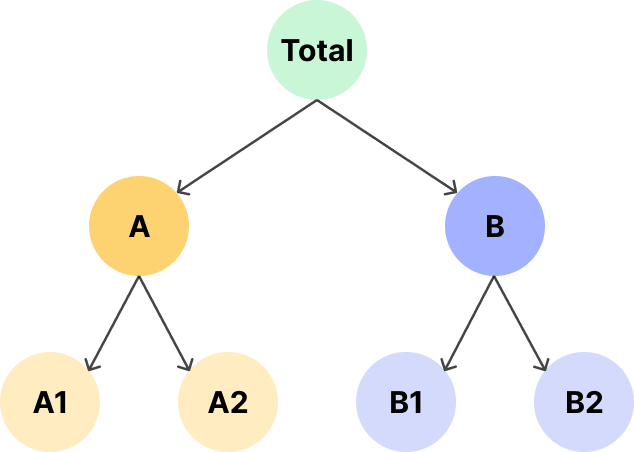
\includegraphics[width=0.4\linewidth,height=\textheight,keepaspectratio]{../figs/hierarchical_structure.png}

}

\caption{\label{fig-hierarchy}A 2-level hierarchical tree structure}

\end{figure}%

The bottom-level (or most disaggregated) series are denoted as
\(\boldsymbol{b}_t \in \mathbb{R}^{n_b}\). Thus, the full vector of all
series in the hierarchy can be represented as:

\[
\boldsymbol{y}_t = \boldsymbol{S} \boldsymbol{b}_t,
\]

where \(\boldsymbol{S} \in \mathbb{R}^{n \times n_b}\) is a summing
matrix that aggregates the bottom-level to all-level series. The summing
matrix \(\boldsymbol{S}\) for the tree structure in
Figure~\ref{fig-hierarchy} is:

\[
\boldsymbol{S} = 
\left[
\begin{array}{cccc}
1 & 1 & 1 & 1 \\
1 & 1 & 0 & 0 \\
0 & 0 & 1 & 1 \\
\multicolumn{4}{c}{\boldsymbol{I_4}}
\end{array}
\right],
\]

where \(\boldsymbol{I_4}\) is the \(4 \times 4\) identity matrix. The
matrix \(\boldsymbol{S}\) encodes the aggregation constraints implied by
the structure. Hence, the columns of \(\boldsymbol{S}\) span a linear
subspace. Any observation \(\boldsymbol{y}_t\) that lies inside this
subspace is called \emph{coherent}, while those outside are
\emph{incoherent}. We refer to the subspace spanned by
\(\boldsymbol{S}\) as the \emph{coherent subspace}
\(\mathfrak{s} \in \mathbb{R}^{n_b}\).

This representation extends beyond hierarchical (nested) structures.
When attributes of interest are crossed, such as the company sales at
any aggregation level (company-wise, city-wise, or outlet-wise) is also
considered by kinds of products, the structure is described as a
\emph{grouped structure}. In grouped systems, as illustrated in
Figure~\ref{fig-grouped}, aggregation and disaggregation paths are not
unique, but the linear constraints can still be written compactly
through a summing matrix \(\boldsymbol{S}\). For simplicity, we refer to
both structures as hierarchical structure and distinguish between them
when needed.

\begin{figure}

\centering{

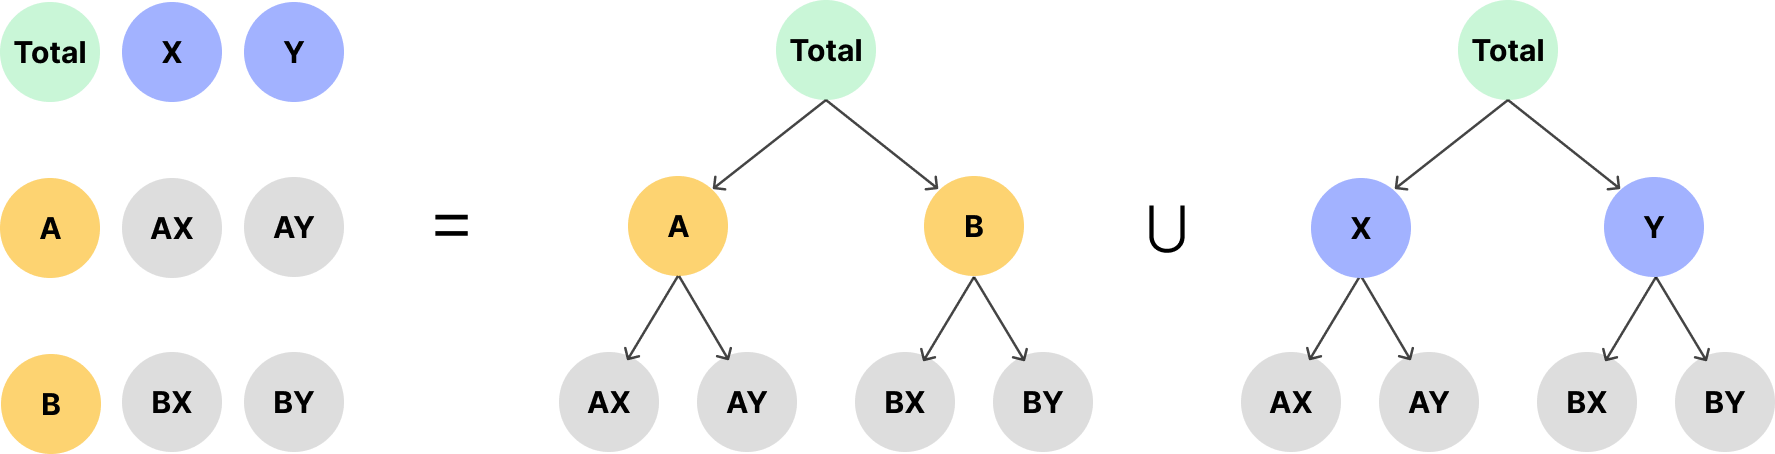
\includegraphics[width=0.9\linewidth,height=\textheight,keepaspectratio]{../figs/grouped_structure.png}

}

\caption{\label{fig-grouped}A 2-level grouped structure, which can be
considered as the union of two hierarchical trees with common top and
bottom level series}

\end{figure}%

In practice, when we produce \(h\)-step-ahead forecasts for each
individual series, referred to as \emph{base forecasts}
\(\hat{\boldsymbol{y}}_{t+h|t}\), they generally violate the aggregation
constraints, and thus are incoherent. Coherency can be restored by
linearly projecting the base forecasts onto the coherent subspace
\(\mathfrak{s}\) using a projection matrix \(\boldsymbol{P}\):
\(\tilde{\boldsymbol{y}}_{t+h|t} = \boldsymbol{P} \hat{\boldsymbol{y}}_{t+h|t}\),
where \(\tilde{\boldsymbol{y}}_{t+h|t}\) are \(h\)-step-ahead
\emph{reconciled forecasts}.

Many existing reconciliation methods including the OLS from Hyndman et
al. (\citeproc{ref-Hyndman2011-jv}{2011}), WLS from Hyndman et al.
(\citeproc{ref-Hyndman2016-ic}{2016}), and MinT from Wickramasuriya et
al. (\citeproc{ref-Wickramasuriya2019-xq}{2019}) express the projection
matrix as \(\boldsymbol{P} = \boldsymbol{S} \boldsymbol{G}\), for a
suitable \(n_b \times n\) mapping matrix \(\boldsymbol{G}\). The role of
this matrix is to map the base forecasts of all levels
\(\hat{\boldsymbol{y}}_{t+h|t}\) down into the bottom level, which is
then aggregated to the higher levels by premultiplying with
\(\boldsymbol{S}\). Since the projection matrix \(\boldsymbol{P}\) is
idempotent, \(\boldsymbol{G}\) must satisfy the condition
\(\boldsymbol{S} \boldsymbol{G} \boldsymbol{S} = \boldsymbol{S}\).
Within this class, a broad family of mapping matrices is given by:
\(\boldsymbol{G} = (\boldsymbol{S}' \boldsymbol{M}^{-1} \boldsymbol{S})^{-1} \boldsymbol{S}' \boldsymbol{M}^{-1}\),
for some positive definite matrix
\(\boldsymbol{M} \in \mathbb{R}^{n \times n}\)
(\citeproc{ref-Gamakumara2020-ml}{Gamakumara, 2020}).

When setting \(\boldsymbol{M} = \boldsymbol{I}_n\), the identity matrix,
the \(\boldsymbol{P}\) matrix reduces to the OLS reconciliation, which
corresponds to an orthogonal projection onto \(\mathfrak{s}\). For a
general positive definite matrix \(\boldsymbol{M}\), \(\boldsymbol{P}\)
is idempotent but not necessarily symmetric, resulting in an oblique
projection. Thus, the choice of \(\boldsymbol{M}\) determines the
projection direction and, in turn, how disagreements among levels are
resolved.

\begin{figure}

\centering{

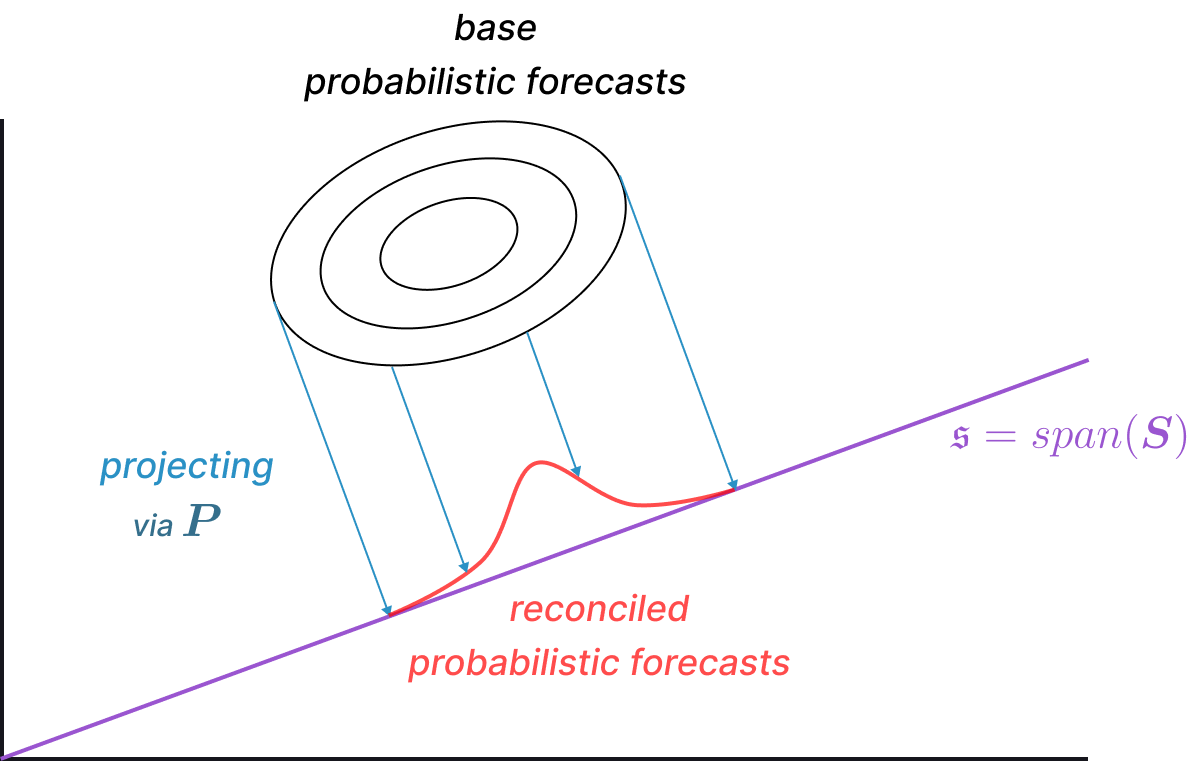
\includegraphics[width=0.6\linewidth,height=\textheight,keepaspectratio]{../figs/geometry_orthogonal.png}

}

\caption{\label{fig-geometry}Geometry of probabilistic forecast
reconciliation. The base forecast distribution is projected orthogonally
onto the coherent subspace (purple line), resulting in the reconciled
forecast distribution (red). The projection is defined by the projection
matrix \(\boldsymbol{P}\). Note that this figure is a schematic since
most applications are high-dimensional.}

\end{figure}%

This projection view extends seamlessly from point to probabilistic
forecast reconciliation. Let \(\hat{\boldsymbol{Y}}_{t+h|t}\) denote the
random vector representing the \(h\)-step-ahead base forecasts. The
random reconciled forecast vector is obtained similarly via projection:
\(\tilde{\boldsymbol{Y}}_{t+h|t} = \boldsymbol{P} \hat{\boldsymbol{Y}}_{t+h|t}\).
Consequently, point forecasts (which we refer to as means of the
predictive distributions) reconcile as
\(\mathbb{E}(\tilde{\boldsymbol{Y}}_{t+h|t}) = \mathbb{E}(\boldsymbol{P} \hat{\boldsymbol{Y}}_{t+h|t}) = \boldsymbol{P} \hat{\boldsymbol{y}}_{t+h|t} = \tilde{\boldsymbol{y}}_{t+h|t}\),
and the covariance of the predictive distribution transforms linearly as
\(\text{Var}(\tilde{\boldsymbol{Y}}_{t+h|t}) = \text{Var}(\boldsymbol{P} \hat{\boldsymbol{Y}}_{t+h|t}) = \boldsymbol{P} \boldsymbol{W}_h \boldsymbol{P}'\),
where \(\boldsymbol{W}_h = \text{Var}(\hat{\boldsymbol{Y}}_{t+h|t})\).

Figure~\ref{fig-geometry} schematically illustrates this projection.
Reconciliation takes the (possibly elliptical) base forecast
distribution and ``pushes'' the entire mass linearly onto the coherent
subspace, resulting in the reconciled forecast distribution.

\subsection{The Minimum Trace
Reconciliation}\label{the-minimum-trace-reconciliation}

Wickramasuriya et al. (\citeproc{ref-Wickramasuriya2019-xq}{2019})
showed that by setting
\(\boldsymbol{M} = \boldsymbol{W}_h = \mathbb{E}( \hat{\boldsymbol{e}}_{t+h|t} \; \hat{\boldsymbol{e}}_{t+h|t}' )\),
the covariance matrix of the \(h\)-step-ahead base forecast errors
\(\hat{\boldsymbol{e}}_{t+h|t} = \boldsymbol{y}_{t+h} - \hat{\boldsymbol{y}}_{t+h|t}\),
we essentially minimise the total variance of the reconciled forecast
errors across all series. Equivalently, MinT is the unique
linear-unbiased reconciler that minimises the trace of
\(\text{Var}[\boldsymbol{y}_{t+h} - \tilde{\boldsymbol{y}}_{t+h|t}] = \boldsymbol{S} \boldsymbol{G}_h \boldsymbol{W}_h \boldsymbol{G}_h' \boldsymbol{S}'\).
This method is thus called Minimum Trace (MinT) reconciliation. The
matrix \(\boldsymbol{G}_h\) is thus given by:

\[
\boldsymbol{G}_h = (\boldsymbol{S}' \boldsymbol{W}_h^{-1} \boldsymbol{S})^{-1}
\boldsymbol{S}' \boldsymbol{W}_h^{-1},
\]

provided that \(\boldsymbol{W}_h\) is positive definite.

Although originally developed for point reconciliation, Wickramasuriya
(\citeproc{ref-Wickramasuriya2024-mb}{2024}) showed that MinT extends
naturally to the probabilistic setting when base predictive
distributions are Gaussian. If \(h\)-step-ahead base forecast
distribution is
\(\mathcal{N}(\hat{\boldsymbol{y}}_{t+h|t}, \boldsymbol{W}_h)\), then
reconciliation gives
\(\tilde{\boldsymbol{Y}}_{t+h|t} = \boldsymbol{S} \boldsymbol{G}_h \hat{\boldsymbol{Y}}_{t+h|t} \sim \mathcal{N}(\tilde{\boldsymbol{y}}_{t+h|t}, \boldsymbol{S} \boldsymbol{G}_h \boldsymbol{W}_h \boldsymbol{G}_h' \boldsymbol{S}')\).
Within the class of linear-unbiased reconcilers, MinT also minimises the
negative log score (equivalently, the Gaussian log predictive score) of
the reconciled distribution.

In this paper we adopt the Gaussian framework to compare the impacts of
different covariance estimators for MinT in both point and probabilistic
reconciliation. It is also worth to mention that the methods can be
extended to non-Gaussian settings by bootstrapping
(\citeproc{ref-Gamakumara2020-ml}{Gamakumara, 2020};
\citeproc{ref-Panagiotelis2023-fs}{Panagiotelis et al., 2023}), which is
beyond the scope of this paper.

\subsection{Shrinkage Estimator for
MinT}\label{shrinkage-estimator-for-mint}

The performance of MinT hinges on a reliable, positive-definite estimate
of \(\boldsymbol{W}_h\), which comes in both the mapping matrix
\(\boldsymbol{G}_h\) and the reconciled forecast error variance
\(\boldsymbol{S} \boldsymbol{G}_h \boldsymbol{W}_h \boldsymbol{G}_h' \boldsymbol{S}'\).

However, the covariance matrix \(\boldsymbol{W}_h\) is often not
available in closed-form, and is challenging to estimate in
high-dimensional setting where the number of series \(n\) is larger than
the time dimension \(T\). To tackle this issue, the original paper by
Wickramasuriya et al. (\citeproc{ref-Wickramasuriya2019-xq}{2019})
assumed a proportionality relationship
\(\hat{\boldsymbol{W}}^g_h = k_h g( \hat{\boldsymbol{W}}_1 )\), where
\(\hat{\boldsymbol{W}}_1\) is the sample covariance matrix of the
in-sample 1-step-ahead base forecast errors (to approximate
\(\boldsymbol{W}_1\)) and \(k_h > 0\) is a scaling constant (which will
be algebraically cancelled out in point-forecast reconciliation). The
function \(g(.)\) is a covariance estimator that produces a
positive-definite matrix, the main focus of this paper.

The recommended choice for \(g(.)\) in the original work is the
shrinkage estimator with diagonal target from Schäfer \& Strimmer
(\citeproc{ref-Schafer2005-yw}{2005}):

\[
\hat{\boldsymbol{W}}^{S}_{1} = \lambda_S \, \boldsymbol{D}_1 + (1 - \lambda_S) \hat{\boldsymbol{W}}_1 \, ,
\]

where \(\boldsymbol{D}_1 = \text{diag}( \hat{\boldsymbol{W}}_1 )\) is
the diagonal matrix comprising the diagonal elements of
\(\hat{\boldsymbol{W}}_1\) (i.e., the sample variances). We refer to any
\(\lambda_S \in [0,1]\) as the shrinkage intensity of the shrinkage
estimator. This approach shrinks the covariance matrix
\(\hat{\boldsymbol{W}}_1\) towards the diagonal target
\(\text{diag}( \hat{\boldsymbol{W}}_1 )\), meaning the off-diagonal
elements are shrunk towards zero while the diagonal ones remain
unchanged.

Schäfer \& Strimmer (\citeproc{ref-Schafer2005-yw}{2005}) also provided
a closed-form estimate of the optimal shrinkage intensity parameter
\(\lambda_S\):

\[
\hat{\lambda}_S = \frac{\sum_{i \neq j} \widehat{Var}(\hat{r}_{ij})} 
{\sum_{i \neq j} \hat{r}_{ij}^2} \, ,
\]

where \(\hat{r}_{ij}\) is the \(i,j\)-th element of
\(\hat{\boldsymbol{R}}_1\), the 1-step-ahead sample correlation matrix
(obtained from \(\hat{\boldsymbol{W}}_1\)). The optimal estimate is
obtained by minimising
\(MSE(\hat{\boldsymbol{W}}_1) = Bias(\hat{\boldsymbol{W}}_1)^2 + Var(\hat{\boldsymbol{W}}_1)\).
More specifically, we trade a small bias for a substantial variance
reduction, which is especially valuable in high dimension.

Despite its simplicity and guaranteed positive-definiteness, MinT
coupled with diagonal-target shrinkage presents three important
limitations.

\subsubsection*{Problem 1: Uniform shrinkage}\label{prob1}
\addcontentsline{toc}{subsubsection}{Problem 1: Uniform shrinkage}

Linear shrinkage shrinks all off-diagonal elements of
\(\hat{\boldsymbol{W}}_1\) towards zeros with equal weights
\(1 - \lambda_S\). The resulting penalty is global and non-adaptive:
strong, genuinely systematic correlations are shrunk at the same rate as
weak, noisy ones. In hierarchical and grouped systems, this can be
problematic. Aggregation naturally induces stronger dependence among
related nodes (for example, a region and a neighbouring region, or a
region and its parent state), while many unrelated pairs exhibit
near-zero correlations. A uniform penalty may over-shrink informative
co-movements or under-shrink idiosyncratic noise, reducing
reconciliation efficiency.

\subsubsection*{Problem 2: Latent factors}\label{prob2}
\addcontentsline{toc}{subsubsection}{Problem 2: Latent factors}

Many real-world hierarchical data sets may exhibit a prominent low-rank
(factor) structure. A clear example is the Australian domestic overnight
trips (\citeproc{ref-tourism-au}{\emph{Tourism Research Australia},
2024}), where the national trips are disaggregated into states and
territories, and further into regions. The tourism activities might be
driven by a few common factors, such as economic conditions, fuel
prices, or major events, which might be left in the forecast errors
after fitting the base models. Figure~\ref{fig-eigen} illustrates the
largest eigenvalues from the one-step forecast error correlation matrix
\(\hat{\boldsymbol{R}}_1\), typically showing a marked elbow after a few
principal components (largest eigenvalues), indicating strong latent
structure. Diagonal-target shrinkage is factor-unaware: it neither
preserves the low-rank common subspace nor differentially shrinks the
idiosyncratic remainder, and so can be inefficient when common factors
dominate.

\begin{figure}

\centering{

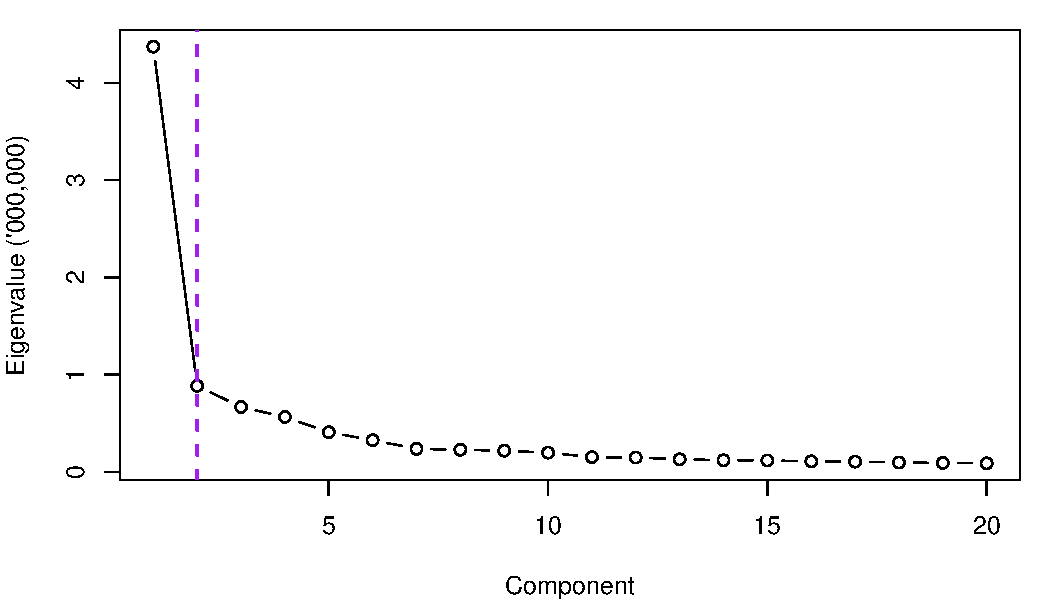
\includegraphics[width=0.7\linewidth,height=\textheight,keepaspectratio]{paper_draft_files/figure-pdf/fig-eigen-1.pdf}

}

\caption{\label{fig-eigen}Scree plot of the eigenvalues of the
1-step-ahead forecast error covariance matrix from the Australian
domestic tourism dataset. The point of inflection occurs around the
second largest eigenvalue.}

\end{figure}%

\subsubsection*{Problem 3: Proportional scaling}\label{prob3}
\addcontentsline{toc}{subsubsection}{Problem 3: Proportional scaling}

The proportionality relationship
\(\hat{\boldsymbol{W}}^g_h = k_h g( \hat{\boldsymbol{W}}_1 )\) enforces
horizon-invariant cross-series dependence of the forecast errors up to a
scalar factor. In many applications, the structure of the error
covariance might change with horizon due to evolving error dynamics or
horizon-specific interactions among series. Proportional scaling may
therefore misrepresent multi-step dependence.

Additionally, while the scalar factor cancels in point reconciliation,
it directly controls dispersion in probabilistic reconciliation and can
lead to miscalibrated predictive distributions. However, we will not
explore this issue in this paper, and leave it for future research.

In the next sections, we introduce alternative covariance estimators
that address these limitations individually and in combination.

\section{Covariance Estimation Approaches}\label{sec-cov-est}

\subsection{NOVELIST Estimator}\label{novelist-estimator}

To tackle the Problem \hyperref[prob1]{1} of uniform shrinkage, we
consider the NOVELIST estimator from Huang \& Fryzlewicz
(\citeproc{ref-Huang2019-ua}{2019}). The NOVELIST (NOVEL Integration of
the Sample and Thresholded Covariance) estimator introduces extra
parameter, the threshold \(\delta\), to control the sparsity level in
the target toward which the sample covariance matrix is shrunk. By
soft-thresholding small correlations before shrinkage, NOVELIST
preserves strong signals while attenuating weak, noisy ones, addressing
the uniform, non-adaptive nature of diagonal-target shrinkage.

The construction proceeds in two steps. First, apply elementwise
soft-thresholding to the sample correlation matrix; second, shrink the
sample correlation toward this thresholded target. The NOVELIST
estimator for covariance matrix is given by:

\[
\hat{\boldsymbol{W}}^{N}_{1} = \lambda_{\delta} \hat{\boldsymbol{W}}_{1, \delta} + (1 - \lambda_{\delta}) \hat{\boldsymbol{W}}_1,
\]

where \(\hat{\boldsymbol{W}}_{1, \delta}\) is the thresholded covariance
matrix of \(\hat{\boldsymbol{W}}_{1}\). As working with correlations
avoids rescaling issues and keeps diagonal entries at one, we rewrite it
in terms of correlations:

\begin{equation}\phantomsection\label{eq-novelist-cor}{
\hat{\boldsymbol{R}}^{N}_{1} = \lambda_{\delta} \hat{\boldsymbol{R}}_{1,\delta} + (1 - \lambda_{\delta}) \hat{\boldsymbol{R}}_1,
}\end{equation}

where, \(\hat{\boldsymbol{R}}_{1,\delta}\) is the thresholded
correlation matrix, where each element is regularised by:

\begin{equation}\phantomsection\label{eq-soft-thr}{
\hat{r}_{1,ij}^\delta = \text{sign}(\hat{r}_{1,ij}) \, 
\text{max}(|\hat{r}_{1,ij}| - \delta, \; 0),
}\end{equation}

where \(\delta \in [0,1]\). For a given threshold \(\delta\), Huang \&
Fryzlewicz (\citeproc{ref-Huang2019-ua}{2019}) derived an analytical
expression for the optimal shrinkage intensity parameter
\(\lambda(\delta)\), following similar logic to Schäfer \& Strimmer
(\citeproc{ref-Schafer2005-yw}{2005}). It can be computed as:

\begin{equation}\phantomsection\label{eq-lambda-thr}{
\hat{\lambda}(\delta) = \frac{
  \sum_{i \neq j} \widehat{Var}(\hat{r}_{1,ij}) \; \boldsymbol{1}(|\hat{r}_{1,ij}| \leq \delta)
} {
  \sum_{i \neq j} (\hat{r}_{1,ij} - \hat{r}_{1,ij}^\delta)^2
},
}\end{equation}

where \(\boldsymbol{1}(.)\) is the indicator function.

On the other hand, the optimal threshold \(\hat \delta\) does not have a
closed-form solution, and is obtained by rolling-window cross-validation
procedure. The idea is to find the threshold \(\delta^*\), with the
corresponding \(\lambda^*\) and
\(\hat{\boldsymbol{R}}^{N}_{1}(\delta^*, \lambda^*)\), that minimises
the average out-of-sample 1-step-ahead mean squared reconciled forecast
errors over all windows. The formal algorithm is given in Algorithm
\ref{alg:novelist_cv}.

Note that when
\(\delta \in \bigl[ \text{max}_{i \neq j}|\hat{r}_{1,ij}|, \; 1 \bigr]\),
the NOVELIST estimator collapses to the shrinkage estimator, and when
\(\delta = 0\), it becomes the sample covariance matrix. An additional
concern is that the estimator is not guaranteed to be positive definite,
but we can use Higham (\citeproc{ref-Higham2002-te}{2002}) algorithm to
compute the nearest positive definite matrix if needed.

\begin{algorithm}[H]
\caption{Cross-validation procedure}\label{alg:novelist_cv}
\begin{algorithmic}[1]

\State \textbf{Input:} Observations and fitted values $\boldsymbol{y}_t, \hat{\boldsymbol{y}}_t \in \mathbb{R}^n$ for $t = 1,\dots,T$ \footnotemark, set of threshold candidates $\Delta$, window size $v$.

\State $\hat{\boldsymbol{e}}_t = \boldsymbol{y}_t - \hat{\boldsymbol{y}}_t$ for $t = 1,\dots,T$

\For{$i = v:T-1$}
    \State $j = i - v +1$
    \State $\hat{\boldsymbol{W}}_1 = \frac{1}{v} \sum_{t=j}^{i} \hat{\boldsymbol{e}}_{t} \hat{\boldsymbol{e}}_{t}'$
    \State $\hat{\boldsymbol{D}} = \text{diag}(\hat{\boldsymbol{W}}_1)$
    \State $\hat{\boldsymbol{R}}_1 = \hat{\boldsymbol{D}}^{-1/2} \hat{\boldsymbol{W}}_1 \hat{\boldsymbol{D}}^{-1/2}$
    \For{$\delta \in \Delta$}
        \State Compute thresholded correlation $\hat{\boldsymbol{R}}_{1,\delta}$ using Equation 2
        \State Compute shrinkage parameter $\hat{\lambda}_{\delta}$ using Equation 3
        \State Compute $\hat{\boldsymbol{R}}^{N}_{1,\delta}$ using Equation 1
        \State $\hat{\boldsymbol{W}}^{N}_{1,\delta} = \hat{\boldsymbol{D}}^{1/2} \hat{\boldsymbol{R}}^{N}_{1,\delta} \hat{\boldsymbol{D}}^{1/2}$
        \State $\boldsymbol{G} = (\boldsymbol{S}' \hat{\boldsymbol{W}}^{N^{-1}}_{1,\delta} \boldsymbol{S})^{-1} \boldsymbol{S}' \hat{\boldsymbol{W}}^{N^{-1}}_{1,\delta}$
        \State Reconciled forecasts $\tilde{\boldsymbol{y}}_{i+1} = \boldsymbol{S} \boldsymbol{G} \hat{\boldsymbol{y}}_{i+1}$
        \State $\tilde{\boldsymbol{e}}_{i+1, \delta} = \boldsymbol{y}_{i+1} - \tilde{\boldsymbol{y}}_{i+1}$
    \EndFor
\EndFor

\State $\text{MSE}_{\delta} = \frac{1}{T-v} \sum_{i=v}^{T-1} (\tilde{\boldsymbol{e}}_{i+1, \delta})^2$ for each $\delta \in \Delta$
\State $\hat{\delta} = \arg\min_{\delta \in \Delta} \text{MSE}_{\delta}$

\State \textbf{Output:} Estimate of optimal threshold parameter $\hat{\delta}$

\end{algorithmic}
\end{algorithm}

\footnotetext{It is only required to fit the base models once on the whole training data $\{\boldsymbol{y}_t\}_{t=1}^T$, and obtain the in-sample fitted values $\{\hat{\boldsymbol{y}}_t\}_{t=1}^T$.}

\vspace{-1em}

\emph{Remark.} Minimising a multi-step-ahead forecast error metric in
the cross-validation procedure oftern yields a \(\hat{\delta}\) that is
close to the 1-step-ahead case.

\subsection{PC-adjusted Estimator}\label{pc-adjusted-estimator}

To address Problem \hyperref[prob2]{2} and exploit latent common
components explicitly, the PC-adjusted (Principal-Component-adjusted)
method takes the latent factors directly into its construction. It
starts by decomposing the covariance matrix \(\hat{\boldsymbol{W}}_1\)
into a prominent principle components part (low-rank) and a orthogonal
complement part \(\hat{\Upsilon}\) (the covariance matrix after removing
the first \(K\) principal components). Then we can apply either
shrinkage or NOVELIST estimator to \(\hat{\boldsymbol{W}}^K_{1}\):

\[
\hat{\boldsymbol{W}}^{g, K}_{1} = \sum_{k = 1}^K \hat{\gamma}_k \hat{\boldsymbol{\xi}}_k \hat{\boldsymbol{\xi}}_k' + g(\hat{\Upsilon})
\]

where \(g(.)\) is either the shrinkage or NOVELIST estimator,
\(\hat{\gamma}_k\) and \(\hat{\boldsymbol{\xi}}_k\) are the \(k\)-th
largest eigenvalue and the corresponding eigenvector of the sample
covariance matrix, respectively.

Similar to the NOVELIST estimator, its PC-adjusted variant
\(\hat{\boldsymbol{W}}^{N, K}_{1}\) requires a cross-validation
procedure to select the threshold paramter and adjustment to obtain
positive definiteness. The reconciled forecasts for each
cross-validation window are obtained using MinT with
\(\hat{\boldsymbol{W}}^{N, K}_{1}\).

\subsection{Scaled Variance}\label{scaled-variance}

To address the potential issue of Problem \hyperref[prob3]{3} of
proportionality relationship
\(\hat{\boldsymbol{W}}^g_h = k_h g( \hat{\boldsymbol{W}}_1 )\) not
holding in practice. A simple relaxation retains the \(1\)-step-ahead
correlation structure but allows the variances to scale differently with
horizon. The scaled variance estimator is given by:

\$\$ \hat{\boldsymbol{W}}\^{}\{g, sv\}\_\{h\} =
\boldsymbol{D}\^{}\{1/2\}\_h \hat{\boldsymbol{R}}\^{}g\_1
\boldsymbol{D}\^{}\{1/2\}\_h, \quad

\hat{\boldsymbol{R}}\^{}g\_1 = D\^{}\{-1/2\}\_1 ,
g(\hat{\boldsymbol{W}}\_1) , D\^{}\{-1/2\}\_1, \$\$

where \(\boldsymbol{D}_h\) is a diagonal matrix comprising
\(\hat{\sigma}^2_{1,h} , \ldots, \hat{\sigma}^2_{n,h}\) on its diagonal,
and \(\hat{\sigma}^2_{i,h}\) is \(h\)-step-ahead base forecast error
variance of the \(i\)-th series. \(\hat{\boldsymbol{R}}^g_1\) is the
estimated one-step correlation matrix using either shrinkage or NOVELIST
estimator.

When NOVELIST is used to produce \(h\)-step-ahead reconciled forecasts,
the cross-validation procedure is modified to evaluate the out-of-sample
\(h\)-step-ahead reconciled forecasts for each window and estimate
optimal threshold parameter (instead of evaluating \(1\)-step-ahead
reconciled forecasts). The reconciled forecasts are obtained using MinT
with \(\hat{\boldsymbol{W}}^{N, sv}_{h}\).

\subsection{Constructing from h-step-ahead
Residuals}\label{constructing-from-h-step-ahead-residuals}

Another alternative is to directly estimate the covariance matrix from
the \(h\)-step-ahead base forecast errors, without assuming any
proportionality relationship:

\[
\hat{\boldsymbol{W}}^{g}_{h} = g(\hat{\boldsymbol{W}}_h),
\]

where \(\hat{\boldsymbol{W}}_h\) is the covariance matrix of in-sample
h-step-ahead base forecast errors, and \(g(.)\) is either the shrinkage
or NOVELIST estimator.

Similarly, if NOVELIST is used, the cross-validation procedure is
modified to evaluate the out-of-sample \(h\)-step-ahead reconciled
forecasts for each window. The reconciled forecasts are obtained using
MinT with \(\hat{\boldsymbol{W}}^{N}_{h}\).

\subsection*{Summary of MinT with Covariance
Estimators}\label{summary-of-mint-with-covariance-estimators}
\addcontentsline{toc}{subsection}{Summary of MinT with Covariance
Estimators}

The covariance estimators explored in this paper are summarised in the
table below. The abbreviations will be used in the following sections.

\begin{longtable}[]{@{}ll@{}}
\caption{Summary of covariance estimators for MinT
reconciliation}\label{tbl-cov}\tabularnewline
\toprule\noalign{}
Covariance estimators used & Abbreviation \\
\midrule\noalign{}
\endfirsthead
\toprule\noalign{}
Covariance estimators used & Abbreviation \\
\midrule\noalign{}
\endhead
\bottomrule\noalign{}
\endlastfoot
Shrinkage & MinT-S \\
NOVELIST & MinT-N \\
PC-adjusted Shrinkage with \emph{K} PCs & MinT-S(PC\emph{K}) \\
PC-adjusted NOVELIST with \emph{K} PCs & MinT-N(PC\emph{K}) \\
Scaled Variance Shrinkage & MinT-S(sv) \\
Scaled Variance NOVELIST & MinT-N(sv) \\
Constructed from h-step-ahead Shrinkage & MinT-S(hcov) \\
Constructed from h-step-ahead NOVELIST & MinT-N(hcov) \\
\end{longtable}

\section{Evaluation of Point and Probabilistic
Forecasts}\label{sec-scores}

This section briefly introduces the scoring rules used to evaluate the
point and probabilistic forecast accuracy in
Section~\ref{sec-simulation} and Section~\ref{sec-empirical}.

For point forecasts, we use the mean squared error (MSE) to evaluate the
accuracy of different reconciliation methods:
\(MSE = \frac{1}{n} \sum_{i=1}^n (y_{i, t+h} - \tilde{y}_{i,t+h|t})^2\),
where \(y_{i, t+h}\) is the realised value of series \(i\) at time
\(t+h\), and \(\tilde{y}_{i,t+h|t}\) is the reconciled point forecast.

Meanwhile, to assess the quality of the probabilistic forecasts, it is
common to use proper scoring rules. A scoring rule is a function
\(S(., .)\) taking a predictive distribution as its first argument and a
realisation as its second argument, then returns a numerical score. We
follow a convention that lower scores are better. A scoring rule is said
to be \emph{proper} if
\(\mathbb{E}_Q[S(Q, y)] \leq \mathbb{E}_Q[S(F, y)]\) for all \(F\),
where \(F\) is a predictive distribution produced by forecasting model,
\(Q\) is the true distribution of the realisation \(y\), and
\(\mathbb{E}_Q\) is the expectation with respect to \(Q\). Hence, the
expected score is minimised when the forecast distribution matches the
true distribution.

We employ Winkler score and continuous ranked probability score as our
univariate scoring rules, and energy score as the multivariate scoring
rule. All three are proper scoring rules. In this paper, we only
evaluate \(1\)-step-ahead probabilistic forecasts, and thus we drop the
subscript \(t\) and \(h\) for simplicity.

\textcolor{blue}{\textit{Winkler score (WS).}} If the
100\((1-\alpha)\)\% prediction interval of \(i\)-th series is
\([l_i, u_i]\) (the \(\alpha / 2\) and \(1 - \alpha / 2\) quantiles),
then the Winkler score is defined as:

\[
WS_{\alpha}(l_i, u_i; y_i) = (u_i - l_i) + \frac{2}{\alpha} (l_i - y_i) \boldsymbol{1}(y_i < l_i) + \frac{2}{\alpha} (y_i - u_i) \boldsymbol{1}(y_i > u_i),
\]

where \(y_i\) is the observed value of \(i\)-th series, and
\(\boldsymbol{1}(.)\) is the indicator function. The Winkler score
rewards narrow intervals that contain the observation, and penalises
intervals that do not contain the observation.

\textcolor{blue}{\textit{Continuous ranked probability score (CRPS).}}
The CRPS is defined as the squared difference between the predictive
cumulative distribution function (CDF) \(F_i\) and the empirical CDF of
the observation \(y_i\) of series \(i\):

\[
CRPS(F_i, y_i) = \int_{-\infty}^{\infty} (F_i(x) - \boldsymbol{1}(x \geq y_i))^2 dx.
\]

When the predictive distribution is Gaussian with mean \(\mu_i\) and
standard deviation \(\sigma_i\), the CRPS has a closed-form expression:

\[
CRPS(F_i, y_i) = \sigma_i \left[ z_i \left( 2 \Phi(z_i) -1 \right) + 2 \phi(z_i) - \frac{1}{\sqrt{\pi}} \right],
\]

where \(z_i = \frac{y_i - \mu_i}{\sigma_i}\), and \(\Phi(.)\) and
\(\phi(.)\) are the CDF and probability density function (PDF) of a
standard normal distribution, respectively.

\textcolor{blue}{\textit{Energy score (ES).}} The energy score is a
multivariate generalisation of the CRPS. It is defined as:

\[
ES(F, \boldsymbol{y}) = \mathbb{E}_F ||\boldsymbol{X} - \boldsymbol{y}||^{\beta} - \frac{1}{2} \mathbb{E}_F ||\boldsymbol{X} - \boldsymbol{X}'||^{\beta},
\]

where \(\boldsymbol{X}\) and \(\boldsymbol{X}'\) are independent random
vectors with multivariate distribution \(F\), \(\boldsymbol{y}\) is the
observed vector, \(||.||\) is the Euclidean norm, and
\(\beta \in (0, 2]\). We set \(\beta = 1\) following common convention.

Since the closed-form expression of the ES may not available, we
approximate it using Monte Carlo samples
\(\{\boldsymbol{x}_1, \ldots, \boldsymbol{x}_M\}\) drawn from \(P\):

\[
\widehat{ES}(F, \boldsymbol{y}) = \frac{1}{M} \sum_{m=1}^M ||\boldsymbol{x}_m - \boldsymbol{y}|| - \frac{1}{2M(M-1)} \sum_{m=1}^M ||\boldsymbol{x}_m - \boldsymbol{x}^*_m||,
\]

where \(\boldsymbol{x}^*_m\) is a randomly selected sample from
\(\{\boldsymbol{x}_1, \ldots, \boldsymbol{x}_M\} \setminus \{\boldsymbol{x}_m\}\).
In our experiments, we use \(M=10000\) samples to approximate the ES.

\section{Simulation}\label{sec-simulation}

\subsection{General Design}\label{general-design}

The general design of data generating process for bottom-level series is
a stationary VAR(1) process, with the following structure:

\[
\boldsymbol{b}_t = \boldsymbol{A} \boldsymbol{b}_{t-1} + \boldsymbol{\epsilon}_t,
\]

where \(\boldsymbol{A}\) is a \(n_b \times n_b\) block diagonal matrix
of autoregressive coefficients
\(\boldsymbol{A} = diag(\boldsymbol{A}_1, \ldots, \boldsymbol{A}_M)\),
with each \(\boldsymbol{A}_m\) being a \(n_{b,m} \times n_{b,m}\)
matrix. The block diagonal structure ensures that the time series are
grouped into \(M\) groups (blocks), with each group having its own
autoregressive coefficients. This aims to simulate the interdependencies
between the time series within each group, where reconciliation will be
expected to better capture these compared to independent base forecasts.

\(\boldsymbol{\epsilon}_t\) is a Gaussian innovation process, with
covariance matrix \(\boldsymbol{\Sigma}\). The covariance matrix
\(\boldsymbol{\Sigma}\) is generated specifically using the Algorithm 1
in Hardin et al. (\citeproc{ref-Hardin2013-wu}{2013}):

\begin{enumerate}
\def\labelenumi{\arabic{enumi}.}
\item
  A compound symmetric correlation matrix is used for each block of size
  \(n_{b,m}\) in \(\boldsymbol{A}_m\), where the correlation entries
  \(\rho_j\) for each block \(m\) are sampled from a uniform
  distribution between 0 and 1. They are within group baseline
  correlations.
\item
  A constant correlation, which is smaller than
  \(\text{min} \{\rho_1, \rho_2, \dots, \rho_M \}\), is imposed on the
  entries between different blocks. It serves as between group baseline
  correlations.
\item
  We select a constant \(\varepsilon\) such that
  \(0 \le \varepsilon < 1 - \text{max} \{\rho_1, \rho_2, \dots, \rho_M \}\)
  to control the noise intensity. We then generate \(n_b\) unit vectors
  \(\boldsymbol{u}_1, \dots, \boldsymbol{u}_{n_b}\) and obtain a
  entry-wise noise element as
  \(\varepsilon \boldsymbol{u}_i' \boldsymbol{u}_j\) for the \(i,j\)-th
  entry. These entry-wise noise elements are added on top of the
  baseline correlation matrix (except the diagonal entries), creating a
  noisy positive correlation matrix \(\boldsymbol{R}^+\).
\item
  The covariance matrix \(\boldsymbol{\Sigma}^+\) is then constructed by
  \(\boldsymbol{\Sigma}^+ = \boldsymbol{D} \boldsymbol{R}^+ \boldsymbol{D}\),
  where \(\boldsymbol{D} = diag(\sigma_1, \dots, \sigma_{n_b})\) is a
  diagonal matrix of standard deviations. Each \(\sigma_i\) is uniformly
  sampled from the range of \([\sqrt{2}, \sqrt{6}]\), for all \(n_b\)
  series.
\end{enumerate}

These steps result in a positive covariance matrix
\(\boldsymbol{\Sigma}^+\) where all the elements are positive. To allow
a mixture of positive and negative covariance, we randomly flip the
signs of them but need to maintain the positive definiteness. This can
be done by pre- and post-multiplying \(\boldsymbol{\Sigma}\) by a random
diagonal matrix \(\boldsymbol{V}\) with diagonal entries sampled from
\(\{-1, 1\}\) with equal probability. The final covariance matrix is
given by
\(\boldsymbol{\Sigma} = \boldsymbol{V} \boldsymbol{\Sigma}^+ \boldsymbol{V}\).

For all hierarchies in our experiments, we simulate two panel lengths,
\(T=54\) (``short'') and \(T=304\) (``long''), reserving the final four
observations as an out-of-sample test set. We perform 500 Monte Carlo
replications for each configuration. In each replication, we fit
univariate ARIMA models to the training observations using the automatic
AICc minimization algorithm of Hyndman \& Khandakar
(\citeproc{ref-Hyndman2008-rf}{2008}), implemented in the
\emph{fabletools} package (\citeproc{ref-O-Hara-Wild2024-we}{O'Hara-Wild
et al., 2024}), generating 1--4-step base forecasts. We then reconcile
the base forecasts using different reconciliation methods, and evaluate
their point and probabilistic forecast accuracy on the test set.

\subsection{Exploring Effects of Hierarchy's
Size}\label{sec-sim-hierarchy-size}

In our main experiments, we examine how MinT combined with the different
estimators perform as the hierarchy expands. We generate synthetic data
from the VAR(1) framework described earlier, varying the number of
bottom‐level series, \(n_b\), across two structures: a ``small''
structure with six groups of six bottom-level series
(\(n_b = 6\)x\(6 = 36\)), and a ``large'' configuration with two groups
of fifty bottom-level series (\(n_b = 2\)x\(50 = 100\)).

In the 36‐series case, each block of six forms a level‐1 aggregate, and
those six aggregates form the total. The 100‐series design employs a
deliberately intricate aggregation path to stress‐test reconciliation
methods. We first sum the one hundred bottom series into ten
intermediate series by grouping them in contiguous blocks of ten. These
ten series are then organised into three level-2 aggregates---four,
three, and four series, respectively---before finally summing to a
single top node. This asymmetric hierarchy creates overlapping
correlation patterns: some level‐2 series share bottom‐level groups,
while others draw from both, emulating practical scenarios such as
regional sales aggregations that span multiple product categories or
overlapping territories. The aggregation paths for both structures are
illustrated in Figure~\ref{fig-sim-structures}.

\begin{figure}

\centering{

\pandocbounded{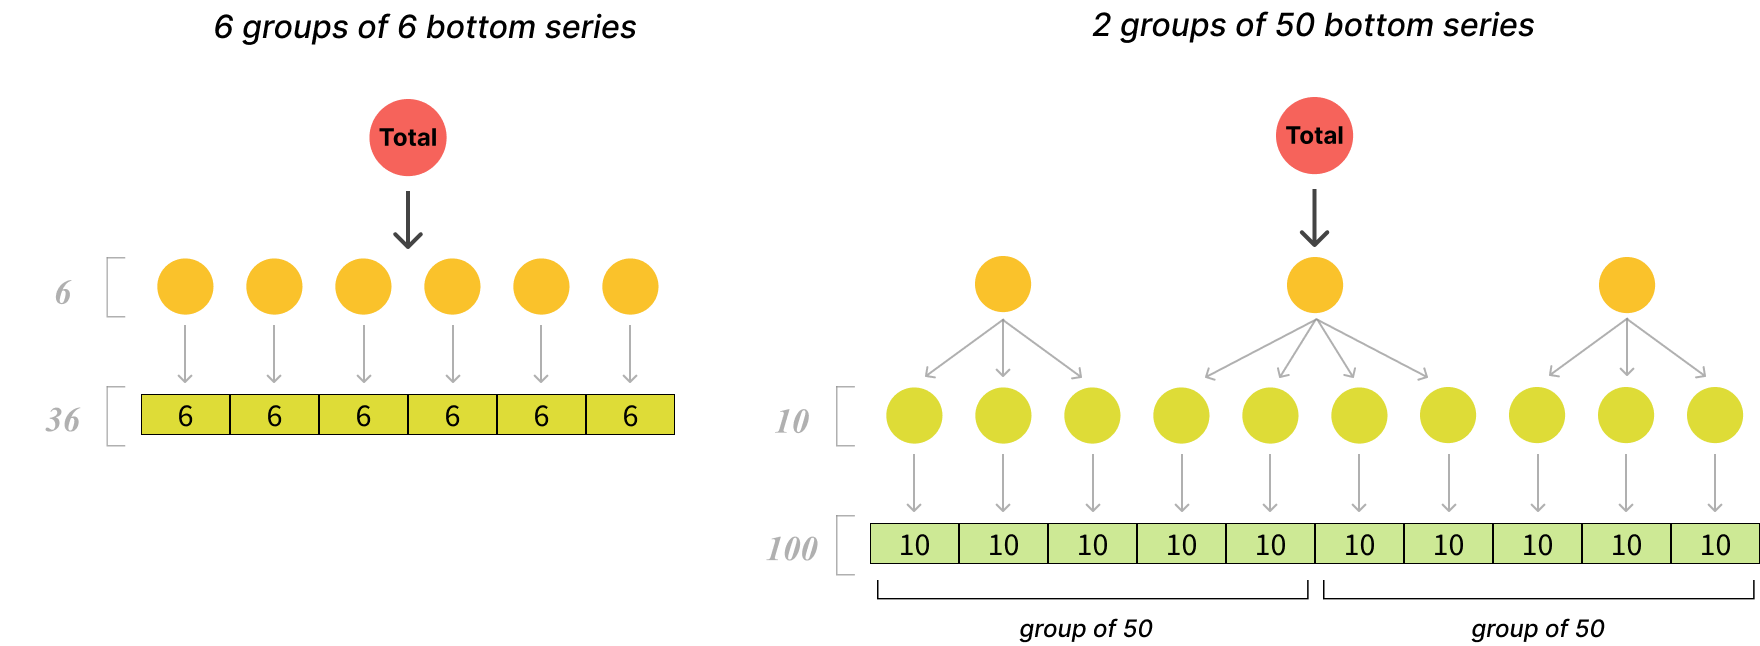
\includegraphics[keepaspectratio]{D:/Github/Recon_Honours_Thesis/figs/sim_structures.png}}

}

\caption{\label{fig-sim-structures}Aggregation structures used in the
simulation experiments: 6 groups of 6 (left) and 2 groups of 50 (right)}

\end{figure}%

The VAR(1) and correlation configurations for the 6 by 6 case and 2 by
50 case are illustrated in Figure~\ref{fig-settings-6x6} and
Figure~\ref{fig-settings-2x50}, respectively. The block diagonal
structure of the VAR(1) coefficient matrices \(\boldsymbol{A}\) reflects
the grouping of series, and the correlation matrices- show higher
correlations among series within the same group.

\begin{figure}

\centering{

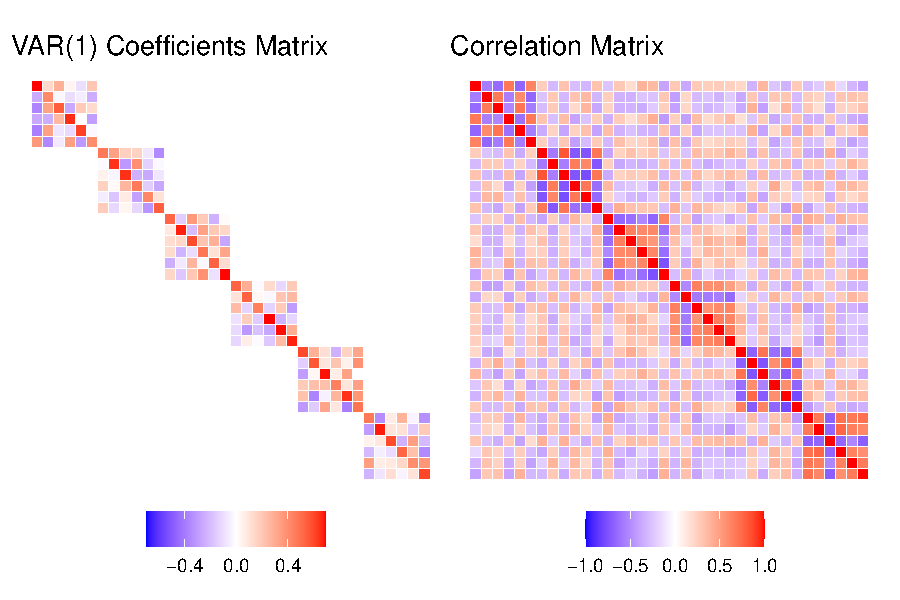
\includegraphics[width=0.75\linewidth,height=\textheight,keepaspectratio]{paper_draft_files/figure-pdf/fig-settings-6x6-1.pdf}

}

\caption{\label{fig-settings-6x6}The VAR(1) coefficients matrix (left)
and correlation matrix of the innovation process (right) for the 6
groups of 6 structure.}

\end{figure}%

\begin{figure}

\centering{

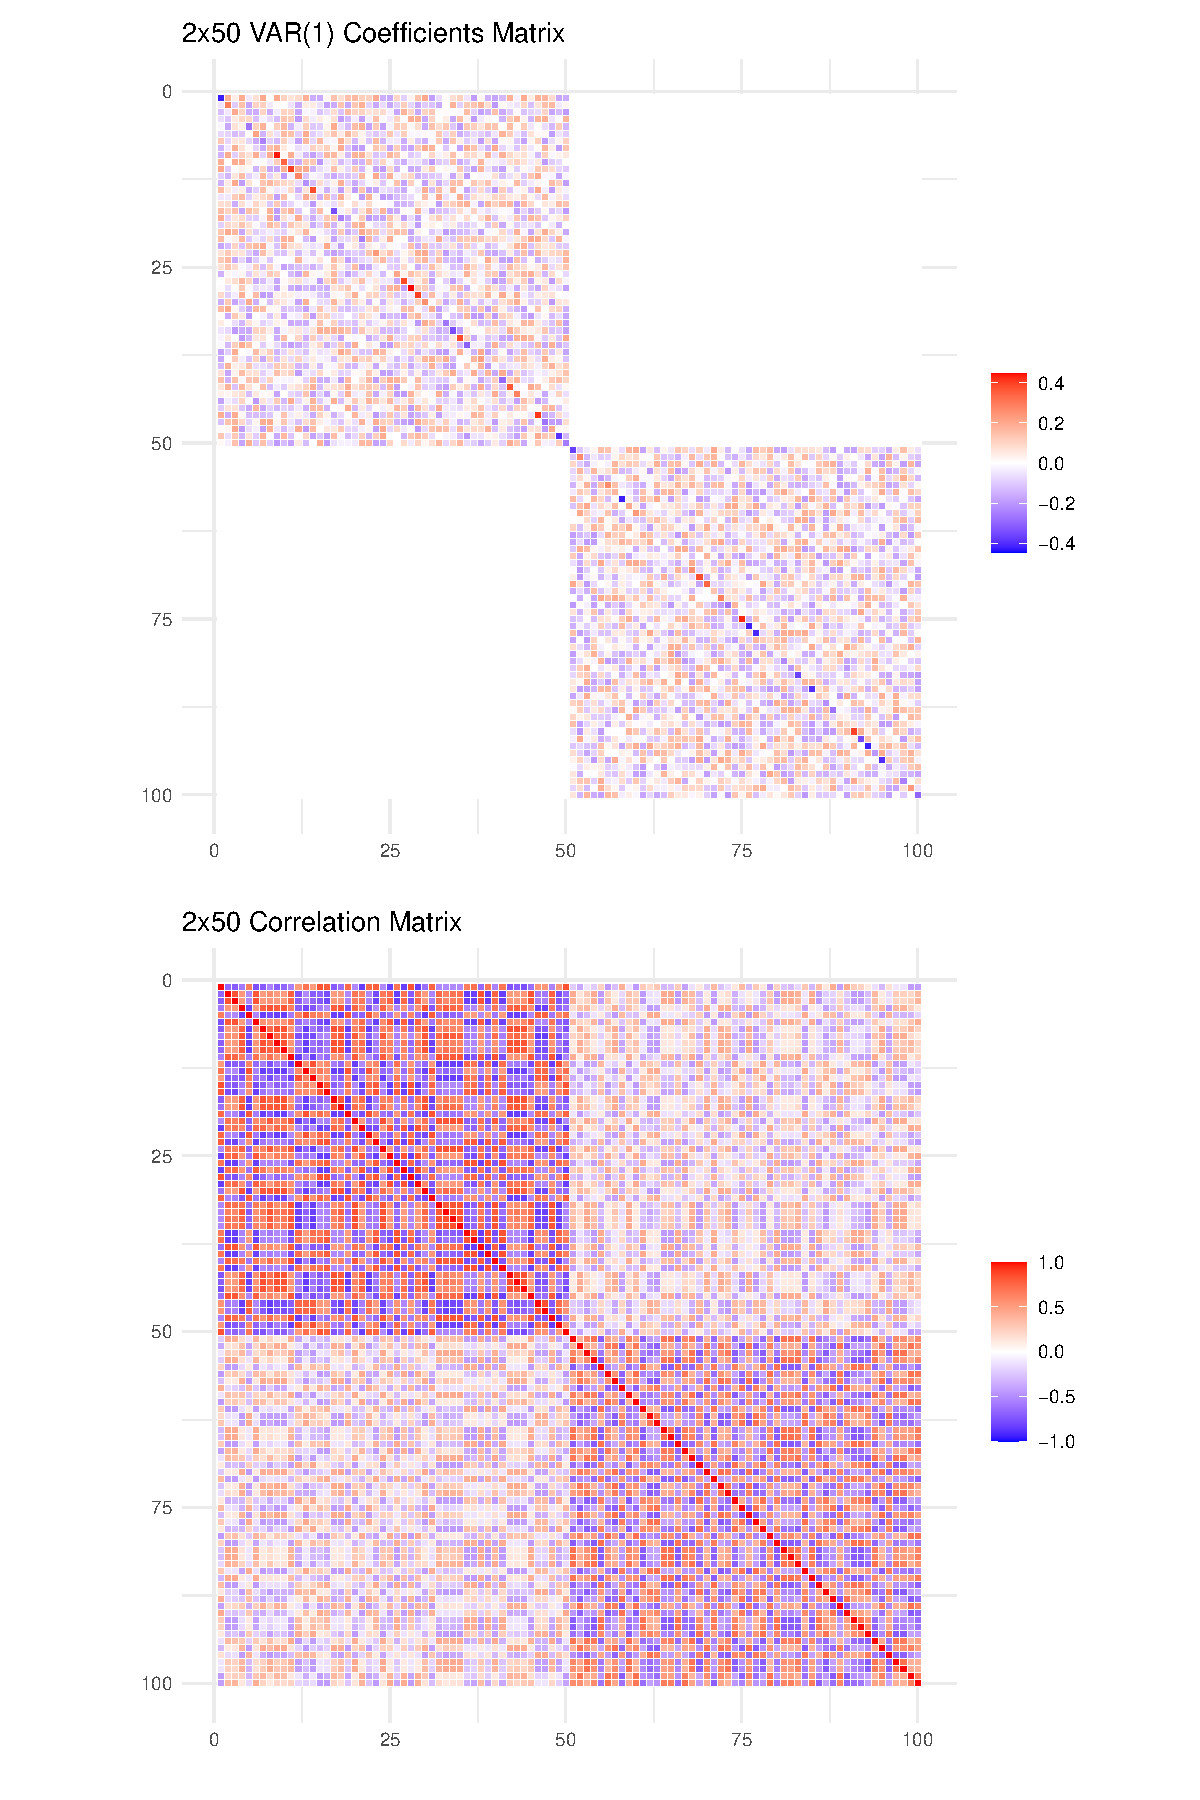
\includegraphics[width=1\linewidth,height=\textheight,keepaspectratio]{paper_draft_files/figure-pdf/fig-settings-2x50-1.pdf}

}

\caption{\label{fig-settings-2x50}The VAR(1) coefficients matrix (top)
and correlation matrix of the innovation process (bottom) for the 2
groups of 50 structure.}

\end{figure}%

\begin{figure}

\centering{

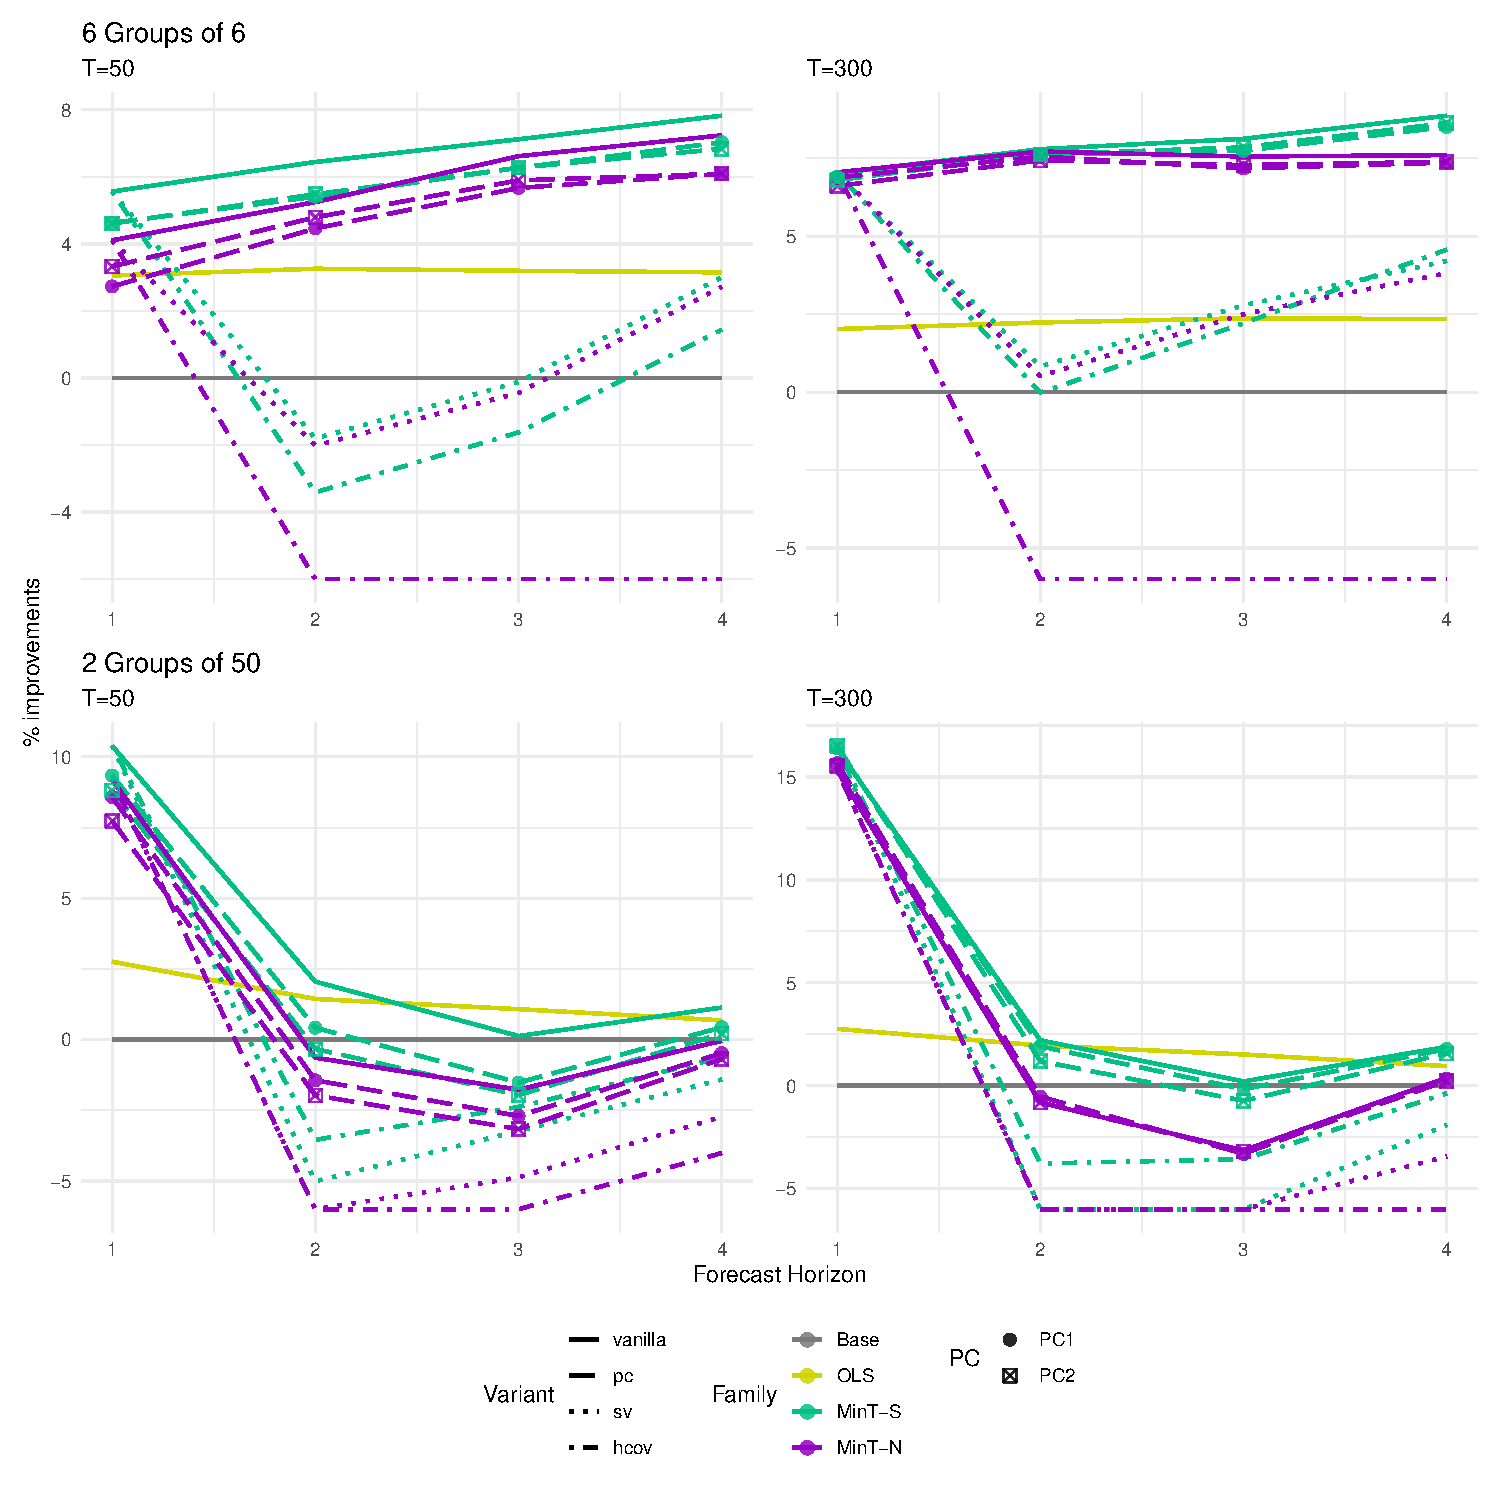
\includegraphics[width=1\linewidth,height=\textheight,keepaspectratio]{paper_draft_files/figure-pdf/fig-sim-results-1-1.pdf}

}

\caption{\label{fig-sim-results-1}Percentage relative improvement in MSE
of reconciled forecasts over the base forecasts in the 6 by 6 case (top
row) and the 2 by 50 case (bottom row), T=50 (left column) and T=300
(right column), for 1- to 4-step-ahead forecasts. The positive
(negative) entries indicate a decrease (increase) in MSE relative to
base. The negative improvements beyond 6\% are capped.}

\end{figure}%

Figure Figure~\ref{fig-sim-results-1} illustrates the relative
improvements in mean squared error (MSE) of reconciled forecasts over
the incoherent base forecasts, across the two structures (small and
large) and time series lengths (short and long). We evaluate ten
different MinT variants based on the covariance estimators discussed in
Table~\ref{tbl-cov}, with visual distinctions made through colors, line
types, and point shapes. MinT with shrinkage (\emph{MinT-S}) and its
variants are colored in mint green, while MinT with NOVELIST
(\emph{MinT-N}) and its variants are in purple. The solid lines
represent vanilla \emph{MinT-S} and \emph{MinT-N}; the dashed lines with
dot points denote the PC-adjusted variants (e.g.~\emph{MinT-S(PC1)},
\emph{MinT-N(PC2)}); and the dotted or dashed-dotted lines indicate the
scaled variance and h-step-ahead residual versions
(e.g.~\emph{MinT-S(SV)}, \emph{MinT-N(hcov)}).

The first key observation is that methods with shrinkage slightly
outperform those with NOVELIST across all scenarios, although the
differences are small. Second, the PC-adjusted variants (using one and
two principal components) do not yield improvements over the vanilla
versions. This is expected since the synthetic data generating process
does not simulate from strong latent factors. Lastly, the scaled
variance and h-step-ahead residual approaches do not enhance performance
as the forecast horizon increases, suggesting that the proportionality
assumption may not be severely violated in this VAR(1) setup.

When looking into each Monte Carlo replication, we find that there are
instances where the NOVELIST estimator collapses to the shrinkage
estimator due to a large optimal threshold \(\hat{\delta}\) being
selected in the cross-validation step, resulting in a diagonal shrinkage
target.

\begin{figure}

\centering{

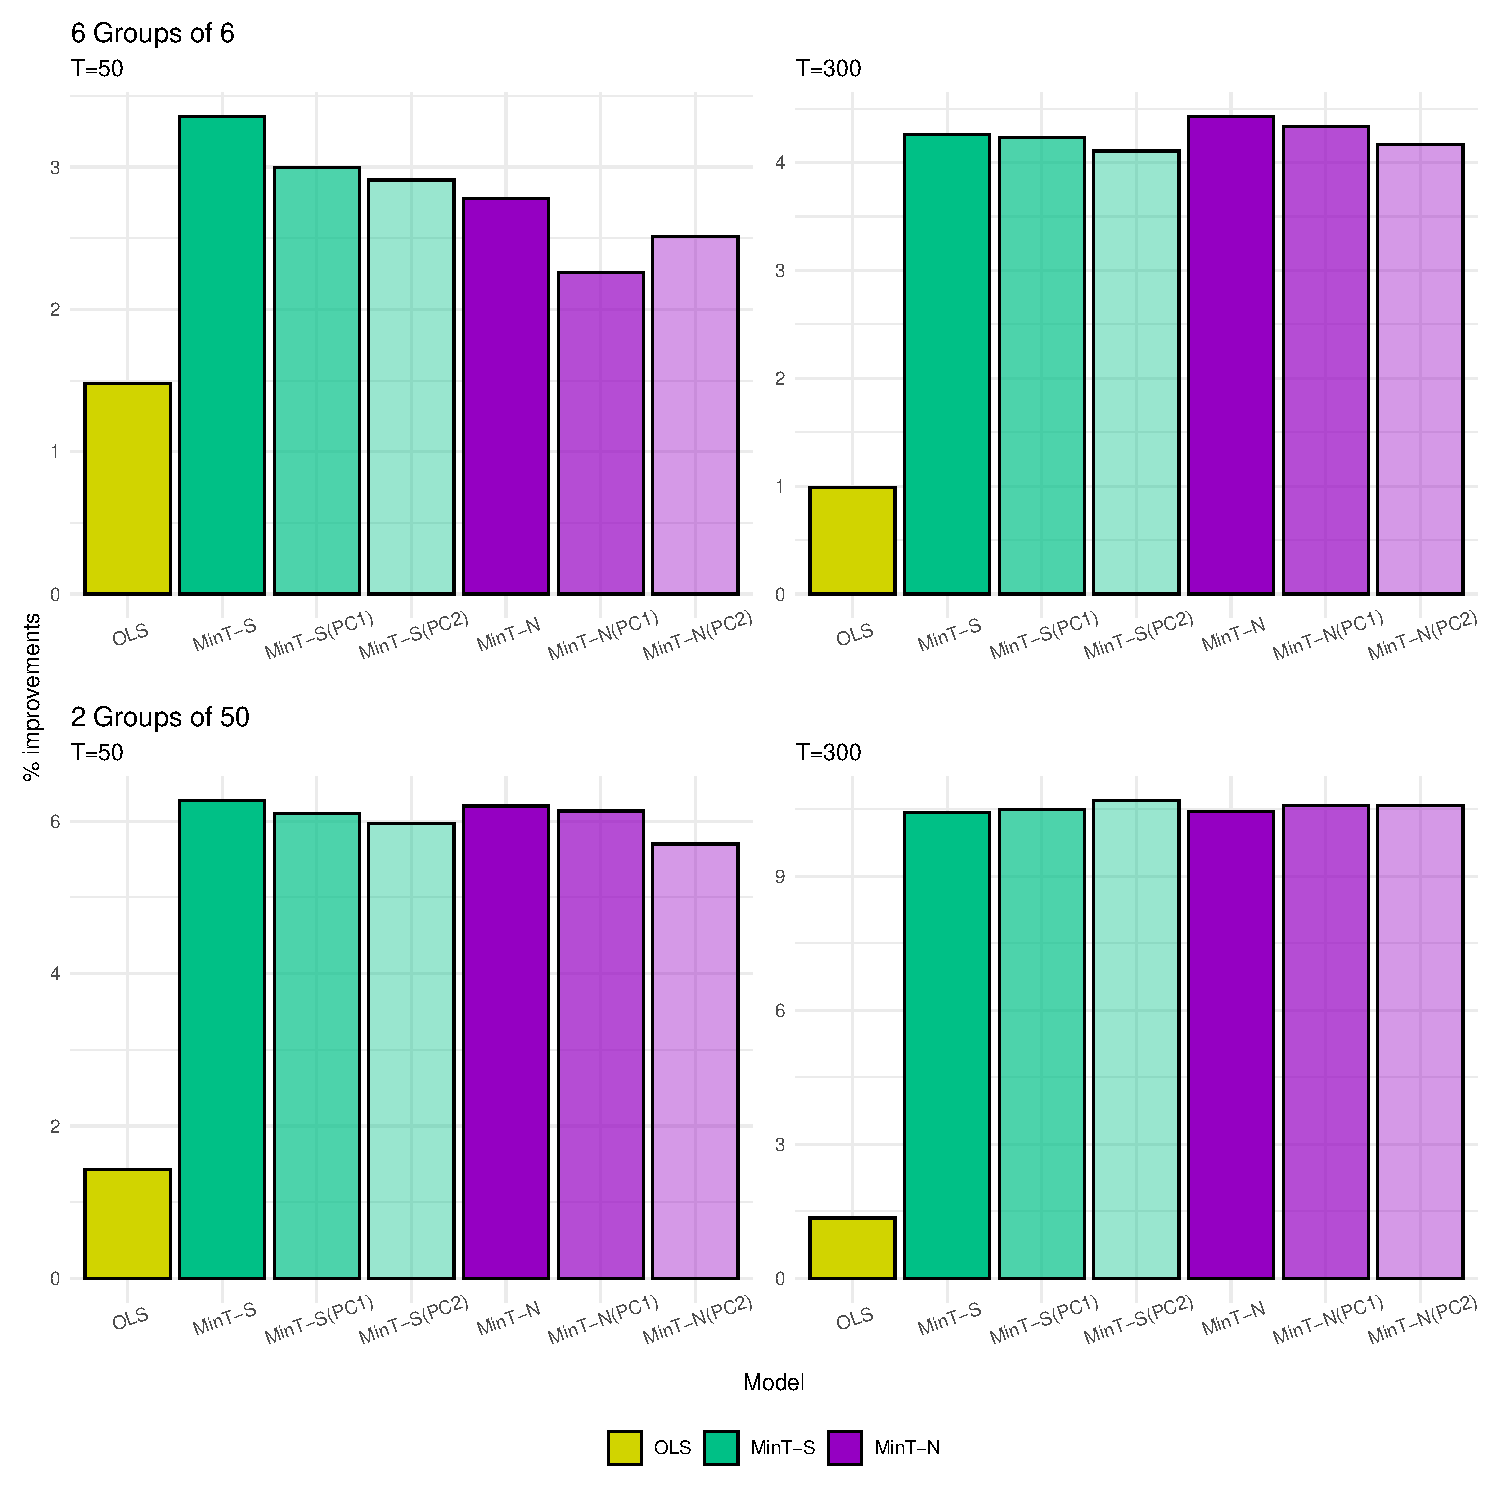
\includegraphics[width=1\linewidth,height=\textheight,keepaspectratio]{paper_draft_files/figure-pdf/fig-sim-results-2-1.pdf}

}

\caption{\label{fig-sim-results-2}Percentage relative improvement in
Energy score in both hierarchies and time dimensions, for 1-step-ahead
forecasts. The positive entries indicate a decrease in Energy score
relative to base.}

\end{figure}%

Moving on to probabilistic forecasts, we evaluate the performance of
reconciliation methods using the energy score, a proper scoring rule for
multivariate predictive distributions. Figure~\ref{fig-sim-results-2}
presents the percentage relative improvement in energy score for
1-step-ahead forecasts. Across both hierarchies and time dimensions, the
MinT methods consistently outperform the base forecasts. Meanwhile, the
differences among \emph{MinT-S} and \emph{MinT-N} variants are small,
except for the 6 by 6 case with 50 observations, where shrinkage has a
pronounced edge. The PC-adjusted variants again degrade performance as
we add more principal components. The scaled variance and h-step-ahead
residuals approaches are not available since we only evaluate
1-step-ahead covariance estimates.

Other scoring rules, such as the Winkler score and CRPS, yield similar
conclusions.

\subsection{Other Data Generating
Processes}\label{other-data-generating-processes}

In attempts to differentiate the performance of NOVELIST from the
shrinkage estimator, we also simulate from a sparse covariance matrix
for the previous section's 2 groups of 50 bottom series setting, as
illustrated in Figure~\ref{fig-Sigma-2x50}. The sparse covariance matrix
is obtained by randomly choosing 40\% of the bottom series and setting
their correlations with all other series to zero, resulting in a
grid-like sparse structure. The VAR(1) coefficient matrix remains the
same as in the dense case. The idea is to allow NOVELIST to exploit the
sparsity in the covariance structure, since it can control the sparsity
of the shrinkage target via the thresholding parameter \(\delta\).
However, no profound insights can be drawn from the results.

\begin{figure}

\centering{

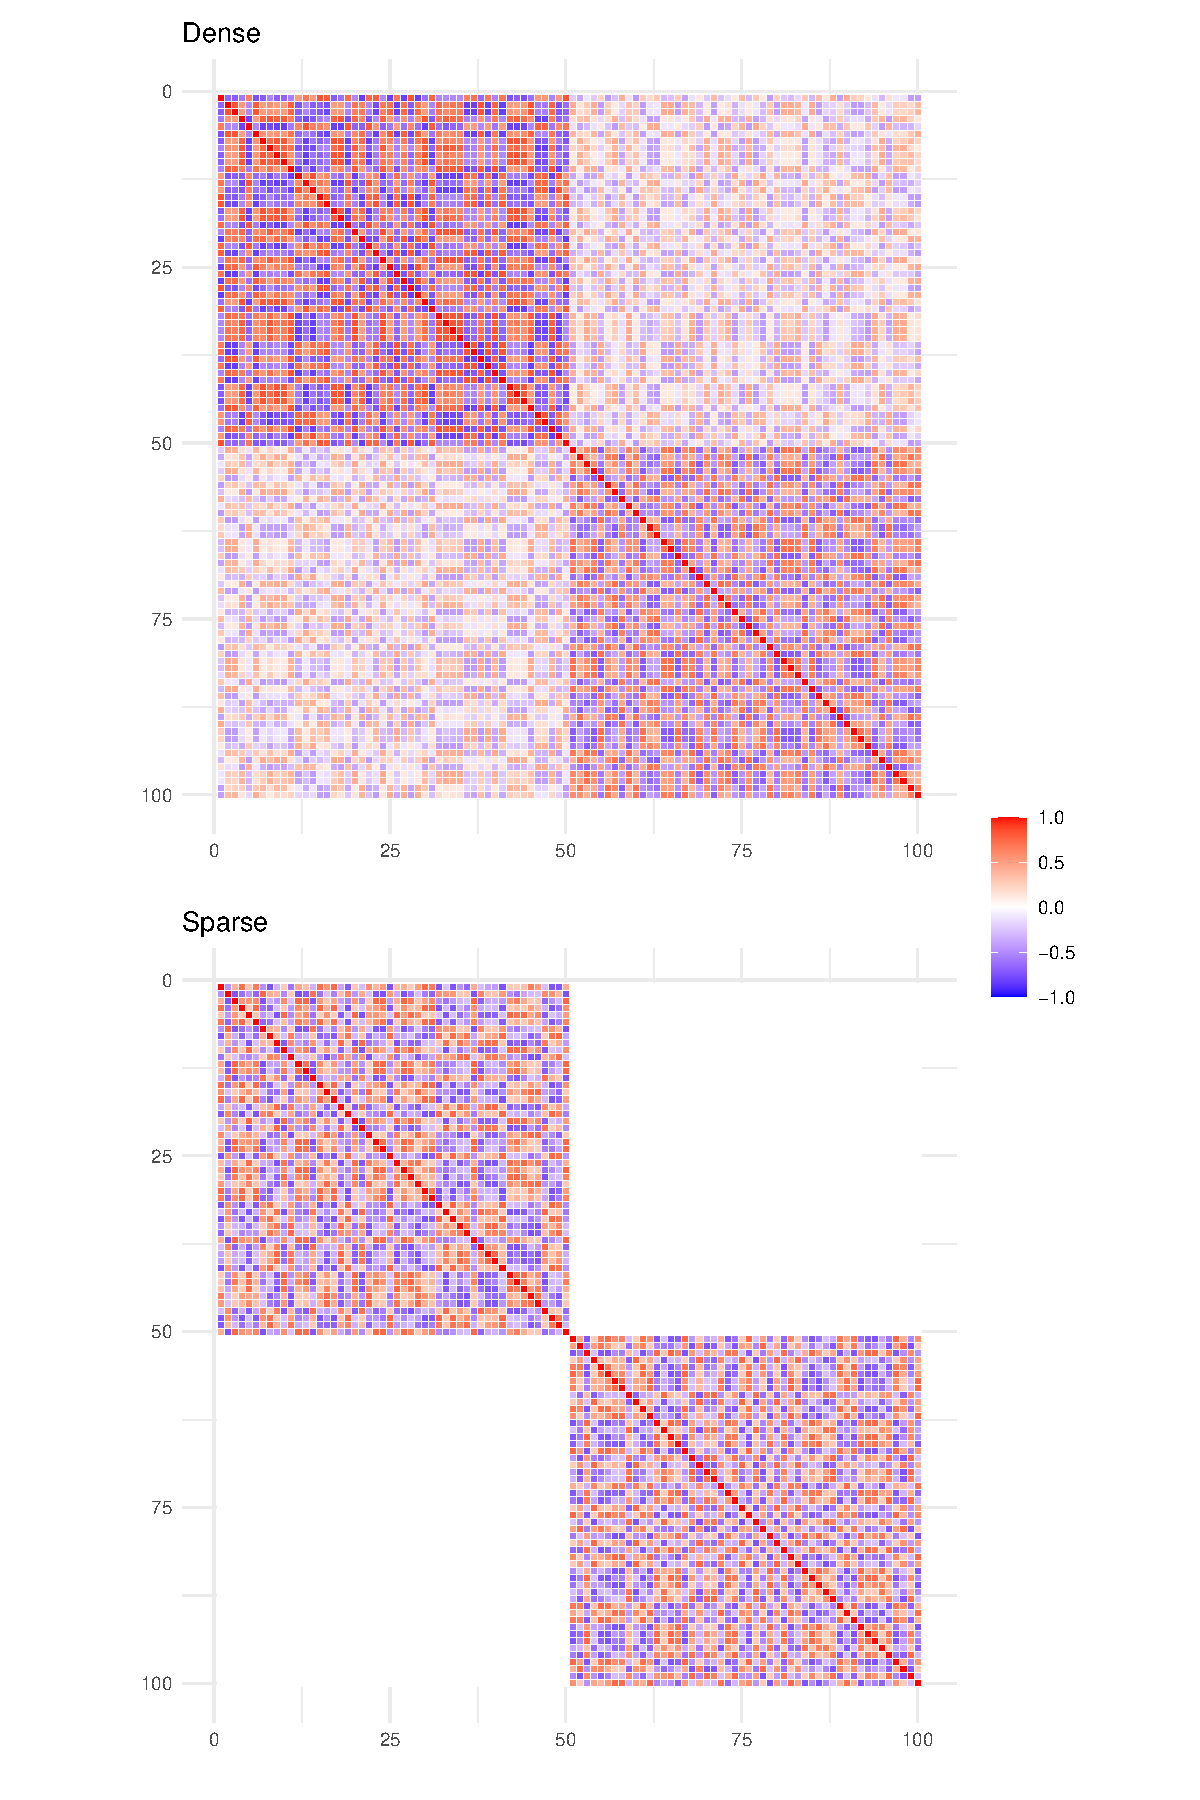
\includegraphics[width=0.8\linewidth,height=\textheight,keepaspectratio]{paper_draft_files/figure-pdf/fig-Sigma-2x50-1.pdf}

}

\caption{\label{fig-Sigma-2x50}Sparse correlation matrix of the
innovation process for 2 groups of 50 structure.}

\end{figure}%

Additional designs (varying block sizes, grouped structure, aggregation
paths, correlation configurations) also failed to separate NOVELIST from
Shrinkage. Their nearly identical performance under these synthetic
scenarios suggests that our current simulation may not unveil the full
advantages of the thresholding estimators. Nevertheless, we have not
explored settings where PC variants or using h-step-ahead residuals
approaches would have an edge.

These findings motivates our turn to empirical data in the next section,
where latent structural features, regime shifts, and noisy, intermittent
series may possibly reveal performance differences.

\section{Forecasting Australian Domestics Tourism}\label{sec-empirical}

Forecasting domestic tourism flows is of great economic and policy
significance, as policymakers and stakeholders rely on accurate
forecasts to make informed decisions regarding resource allocation,
infrastructure development, and marketing strategies. The domestic
tourism flows in Australia exhibit a natural hierarchical and grouped
structure, driven both by geography and by purpose of travel. At the top
of this hierarchy lies the national total, which splits into the seven
states and territories. Each state is further sub-divided into tourism
zones, which in turn break down into 77 regions. A complete illustration
of this geographic hierarchy appears in Appendix
Section~\ref{sec-tourism-supplement}. Intersecting this geographic
hierarchy is a second dimension: policymakers are also interested in
travel motives. This partitions tourism flows into four categories:
holiday, business, visiting friends and relatives, and other.
Altogether, this yields a grouped structure of 560 series, from the most
disaggregated regional-purpose cells up to the full national aggregate.
Table~\ref{tbl-tourism-structure} depicts this structure.

\begin{longtable}[]{@{}
  >{\raggedright\arraybackslash}p{(\linewidth - 6\tabcolsep) * \real{0.1833}}
  >{\centering\arraybackslash}p{(\linewidth - 6\tabcolsep) * \real{0.3667}}
  >{\centering\arraybackslash}p{(\linewidth - 6\tabcolsep) * \real{0.2500}}
  >{\centering\arraybackslash}p{(\linewidth - 6\tabcolsep) * \real{0.2000}}@{}}

\caption{\label{tbl-tourism-structure}Hierarchical and grouped structure
of Australian domestic tourism flows}

\tabularnewline

\toprule\noalign{}
\begin{minipage}[b]{\linewidth}\raggedright
Geographical division
\end{minipage} & \begin{minipage}[b]{\linewidth}\centering
Number of series per geographical division
\end{minipage} & \begin{minipage}[b]{\linewidth}\centering
Number of series per purpose
\end{minipage} & \begin{minipage}[b]{\linewidth}\centering
Total number of series
\end{minipage} \\
\midrule\noalign{}
\endhead
\bottomrule\noalign{}
\endlastfoot
Australia & 1 & 4 & 5 \\
States & 7 & 28 & 35 \\
Zones & 27 & 108 & 135 \\
Regions & 77 & 308 & 385 \\
Total & 112 & 448 & 560 \\

\end{longtable}

We quantify tourism demand via ``visitor nights'', the total number of
nights spent by Australians away from home. The data is collected via
the National Visitor Survey, managed by Tourism Research Australia,
using computer assisted telephone interviews from nearly 120,000
Australian residents aged 15 years and over
(\citeproc{ref-tourism-au}{\emph{Tourism Research Australia}, 2024}).

The data are monthly time series spanning from January 1998 to December
2016, resulting in 228 observations per series. This gives a challenging
high-dimensional forecasting problem with number of series (560) doubled
the number of observations, which is ideal for evaluating reconciliation
approaches that rely on high-dimensional covariance estimation. The
extreme dimensionality over sample size mirrors many contemporary
business problems, for instance, Starbucks Corporation sales. Tourism
demand is also economically vital yet highly volatile, with geographical
and purpose‑specific patterns create a realistic stress‑test for
reconciliation algorithms.

\begin{figure}

\centering{

\includegraphics[width=0.5\linewidth,height=\textheight,keepaspectratio]{D:/Github/Recon_Honours_Thesis/figs/tourism_cv.png}

}

\caption{\label{fig-tourism-cv}Rolling-window cross-validation scheme
for evaluating forecasting performance in Australia tourism data}

\end{figure}%

To assess forecasting performance between models, we adopt a
rolling-window cross-validation scheme. Beginning with the first 120
monthly observations (January 1998-December 2005) as the initial
training set, we obtain the best-fitted ARIMA model for each of the 560
series via the automatic algorithm by minimising AICc from Hyndman \&
Khandakar (\citeproc{ref-Hyndman2008-rf}{2008}), implemented in the
\emph{fabletools} package (\citeproc{ref-O-Hara-Wild2024-we}{O'Hara-Wild
et al., 2024}). The 1- to 12-step-ahead base forecasts are then
generated by these ARIMA models, and then reconciled using multiple
approaches. To estimate the NOVELIST and its variants, we implement an
extra cross-validation prodecure within this training window, as
described in Algorithm \ref{alg:novelist_cv}. We then roll the training
window forward by one month and refit all models, re-estimate
reconciliation variants, and produce another batch of 1- to
12-step-ahead forecasts, repeating until the training set reaches
December 2015. In total, this results in 97 out-of-sample windows. The
entire procedure is illustrated in Figure~\ref{fig-tourism-cv}.

\begin{figure}

\centering{

\pandocbounded{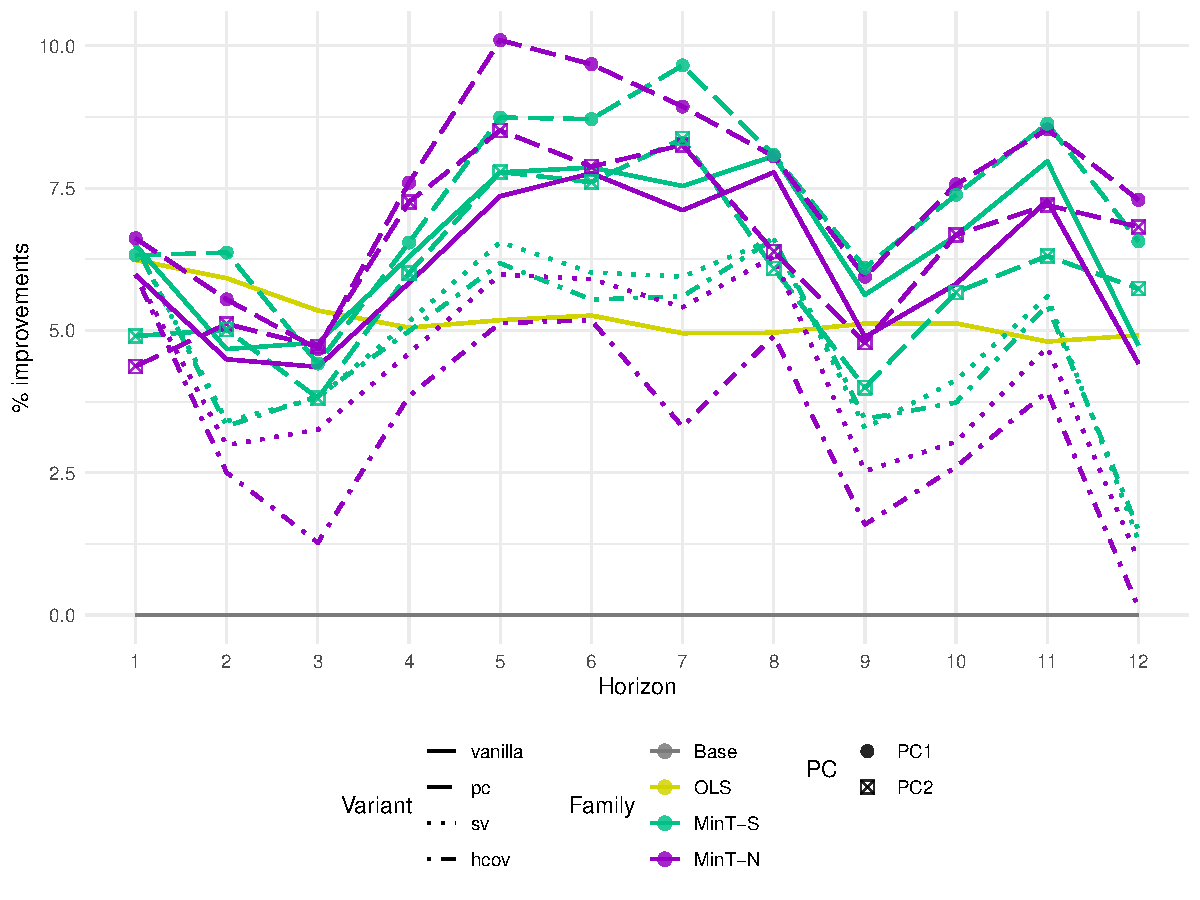
\includegraphics[keepaspectratio]{paper_draft_files/figure-pdf/fig-tourism-MSE-line-1.pdf}}

}

\caption{\label{fig-tourism-MSE-line}Percentage relative improvement in
the mean squared error (MSE) of different reconciled forecasts over the
base forecasts for the Australian domestic tourism data, for 1 to 12
steps ahead forecasts. The positive entries indicate an decrease in
MSE.}

\end{figure}%

\begin{figure}

\centering{

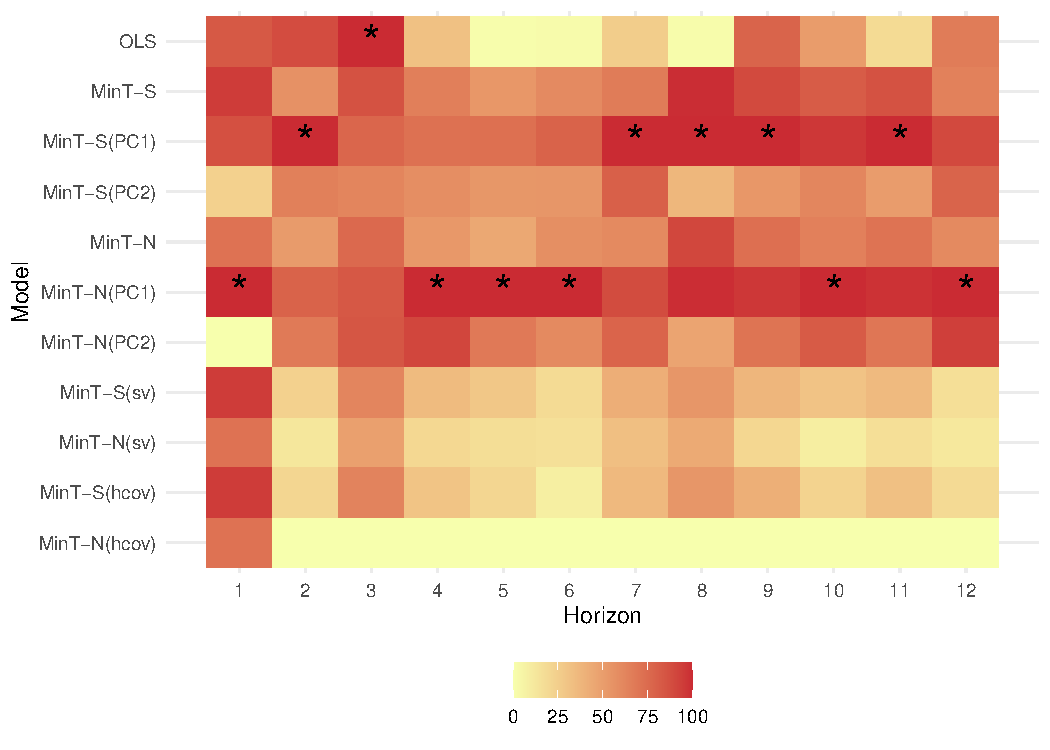
\includegraphics[width=0.9\linewidth,height=\textheight,keepaspectratio]{paper_draft_files/figure-pdf/fig-tourism-MSE-heat-1.pdf}

}

\caption{\label{fig-tourism-MSE-heat}Heatmap of relative improvement in
the mean squared error (MSE) of different reconciled forecasts over the
base forecasts for the Australian domestic tourism data, for 1 to 12
steps ahead forecasts. The values are scaled to the range of 0 to 100
for better visualisation, with darker colors indicating greater
improvement and best performance is noted by a star. This re-scaling
does not affect relative rankings among methods.}

\end{figure}%

Figure~\ref{fig-tourism-MSE-line} reports percentage relative
improvements in MSE of reconciled forecasts over the incoherent base
ARIMA forecasts, across horizons from 1 to 12 months. We evaluate ten
MinT variants (as defined in Table~\ref{tbl-cov}), similar to the
simulation's Figure~\ref{fig-sim-results-1}. The MinT with shrinkage
(\emph{MinT-S}) and its variants are colored in mint green, while MinT
with NOVELIST (\emph{MinT-N}) and its variants are in purple. Solid
lines represent ``vanilla'' \emph{MinT-S} and \emph{MinT-N}; dashed
lines with dot points denote the PC-adjusted variants
(e.g.~\emph{MinT-S(PC1)}, \emph{MinT-N(PC2)}); and dotted or
dashed-dotted lines indicate the scaled variance and h-step-ahead
residual versions (e.g.~\emph{MinT-S(SV)}, \emph{MinT-N(hcov)}).

Three patterns stand out. First, the vanilla \emph{MinT-S} (solid green)
slightly outperform \emph{MinT-N} (solid purple) at most horizons,
although the gap is small. Second, variants that alter the multi-step
covariance, either via scaled variance or direct h-step residual
covariances, underperform standard MinT, suggesting that extra
estimation at horizon \(h>1\) is not rewarded in this empirical
analysis. Most importantly, incorporating a single dominant factor via
PC-adjustment (dashed line with round points) delivers best performance
among all methods. Both \emph{MinT-S(PC1)} and \emph{MinT-N(PC1)}
consistently beat their unadjusted counterparts across horizons.
However, adding more than one PC brings no additional benefit and can
erode performance, likely due to injecting idiosyncratic noise from
weaker components.

Figure~\ref{fig-tourism-MSE-heat} complements the line plot with a
heatmap that standardises each method's MSE improvement to a 0--100
scale to enhance visual discrimination across horizons. Darker shades
indicate larger improvements. The heatmap highlights the pattern from
the line plot: \emph{MinT-N(PC1)} and \emph{MinT-S(PC1)} exhibit the
highest concentration of dark cells and are repeatedly marked as the
best method across horizons (star markers). Overall, the results
underscores the consistent gains from PC adjustment and highlights the
diminishing returns from more complex covariance treatments (lighter
cells for scaled variance and h-step residuals).

\begin{figure}

\centering{

\pandocbounded{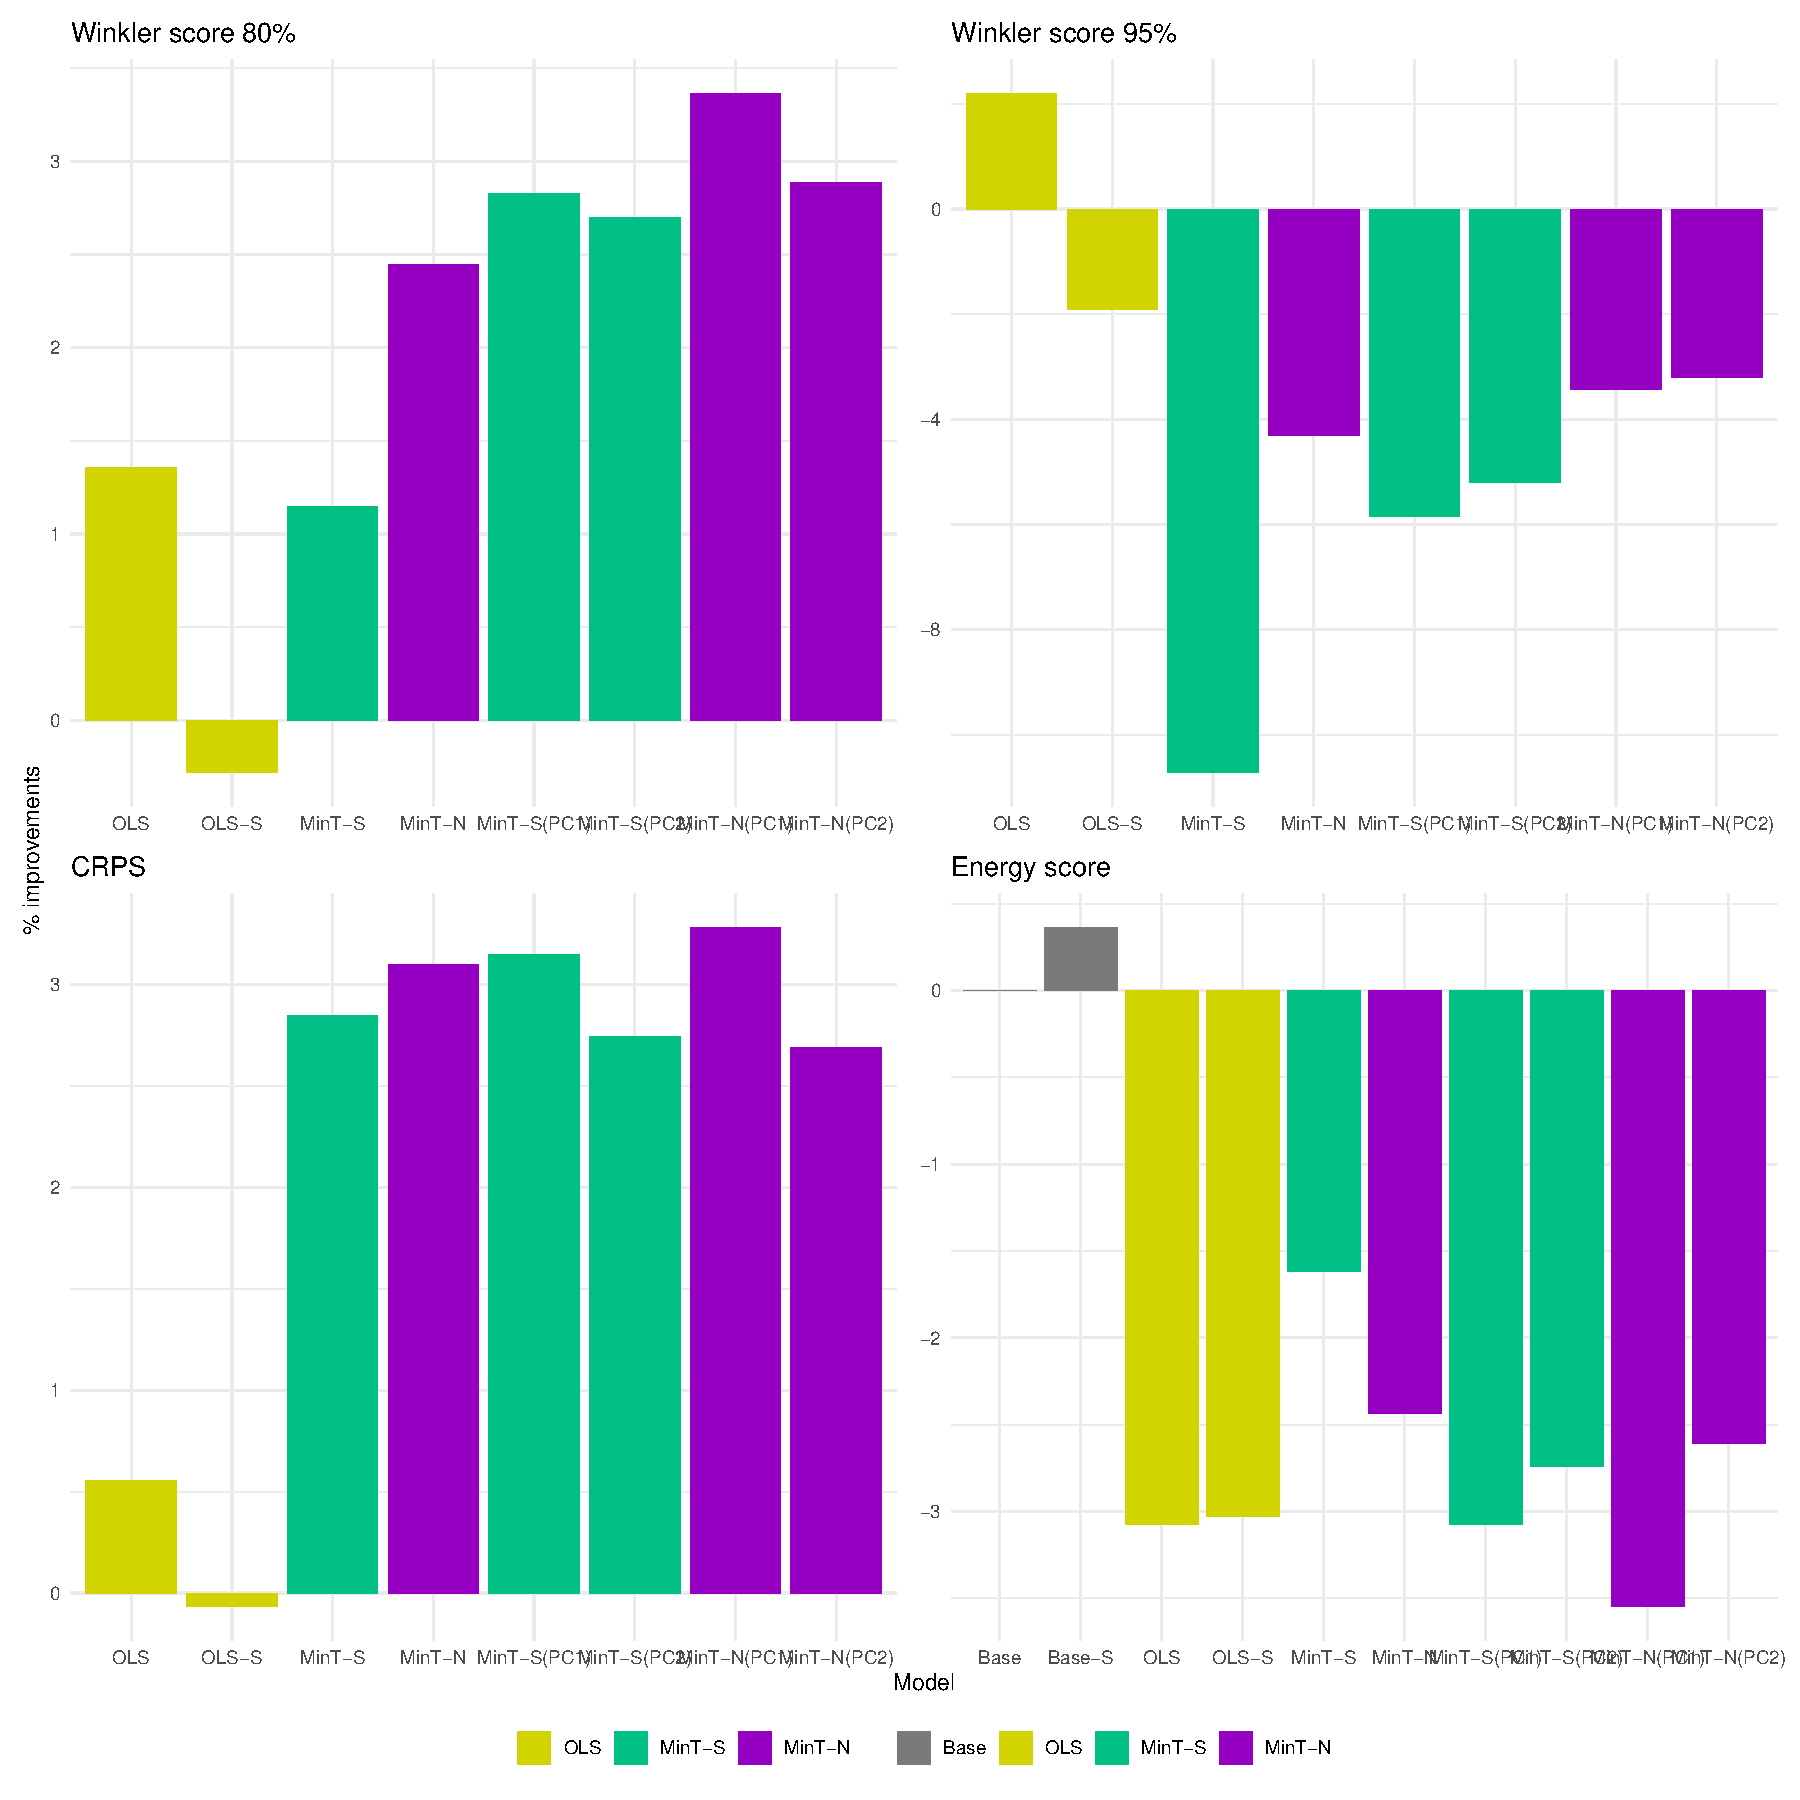
\includegraphics[keepaspectratio]{paper_draft_files/figure-pdf/fig-tourism-probscores-1.pdf}}

}

\caption{\label{fig-tourism-probscores}Percentage relative improvement
in the Winkler score at 80\% and 95\% nominal coverage, CRPS, and Energy
score of multiple reconciled forecasts over the base forecasts for the
Australian domestic tourism data, for 1-step-ahead forecasts. The
positive (negative) entries indicate a decrease (increase) in the
probabilistic scores relative to base.}

\end{figure}%

Turning to probabilistic forecasts (1-step-ahead forecasts),
Figure~\ref{fig-tourism-probscores} shows that \emph{MinT-N} variants
(purple bars) consistently outperform \emph{MinT-S} variants (green
bars) across univariate and multivariate scores. The PC1-adjusted
variants again yield improvements over their vanilla counterparts, with
\emph{MinT-N(PC1)} leading overall. In the multivariate evaluation, the
Energy score places \emph{OLS} close to the PC1-adjusted MinT methods.
One surprising finding is that all MinT variants produce inferior
forecasts compared to the base forecasts when considering 95\% Winkler
score, while \emph{OLS} performs best.

\begin{figure}

\centering{

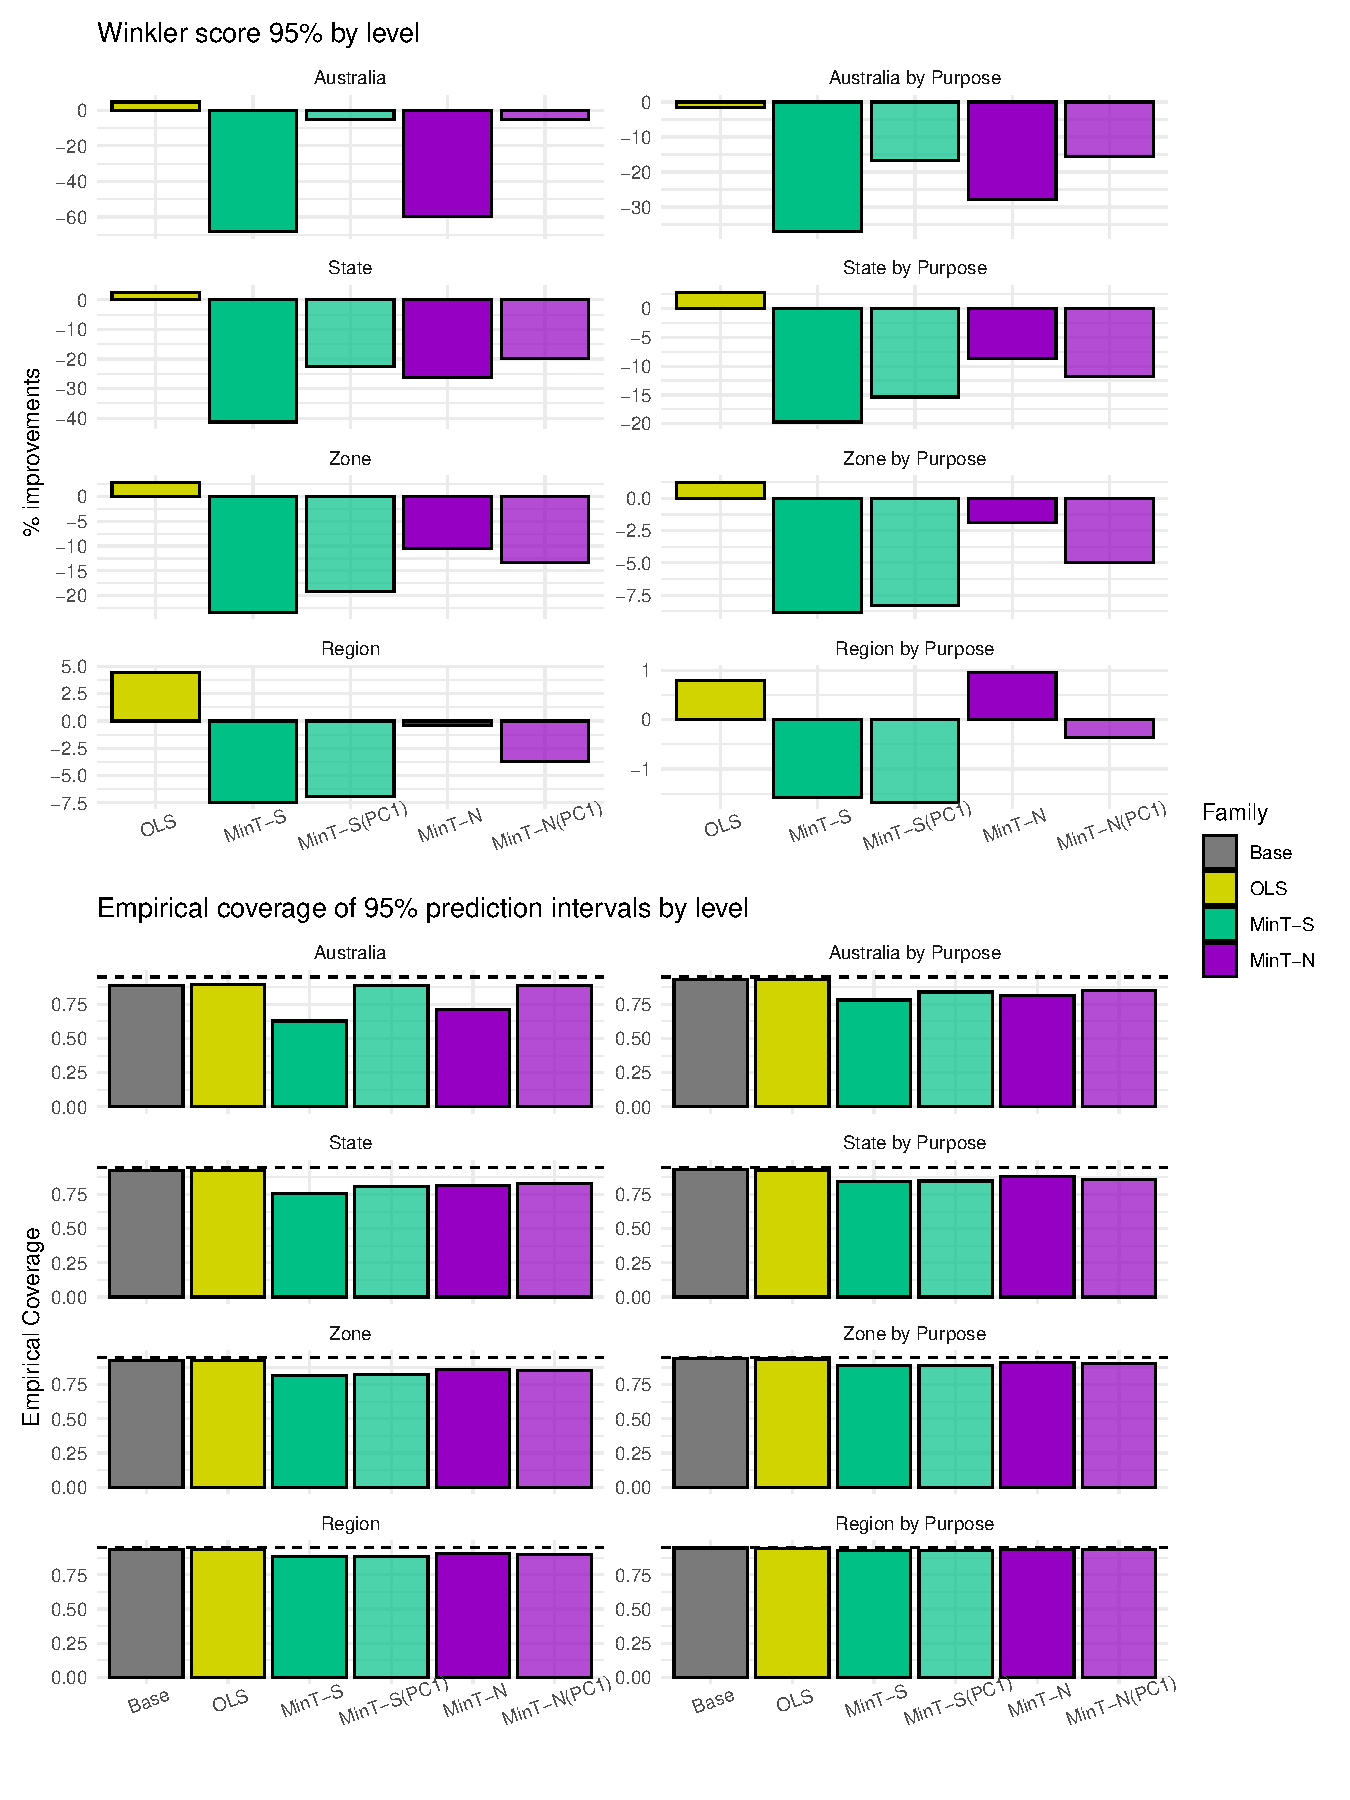
\includegraphics[width=1\linewidth,height=\textheight,keepaspectratio]{paper_draft_files/figure-pdf/fig-tourism-coverage-95-level-1.pdf}

}

\caption{\label{fig-tourism-coverage-95-level}Percentage relative
improvement in Winkler score at 95\% nominal coverage by aggregation
level (left), and empirical coverage of 95\% prediction intervals by
aggregation level (right).}

\end{figure}%

To dissect the 95\% Winkler score results,
Figure~\ref{fig-tourism-coverage-95-level} breaks down performance by
hierarchical level, and examines empirical coverage of the 95\%
prediction intervals. The left panel shows that \emph{MinT-S} produces
inferior forecasts compared to the base forecasts at all levels,
especially in higher aggregated levels. From our inspection, this is due
to the overly shrunk variances from the shrinkage estimator, leading to
narrow prediction intervals. The right panel confirms this, as
\emph{MinT-S} has the lowest empirical coverage across all levels,
indicating that its prediction intervals fail to capture the true
observations adequately and resulting in poor Winkler scores.
\emph{MinT-N} has relatively good coverage and improved Winkler score at
bottom levels, but still is inferior at higher levels. The PC-adjusted
variants seem to strike a better balance, improving overall coverage and
relative Winkler scores over the base.

\begin{figure}

\centering{

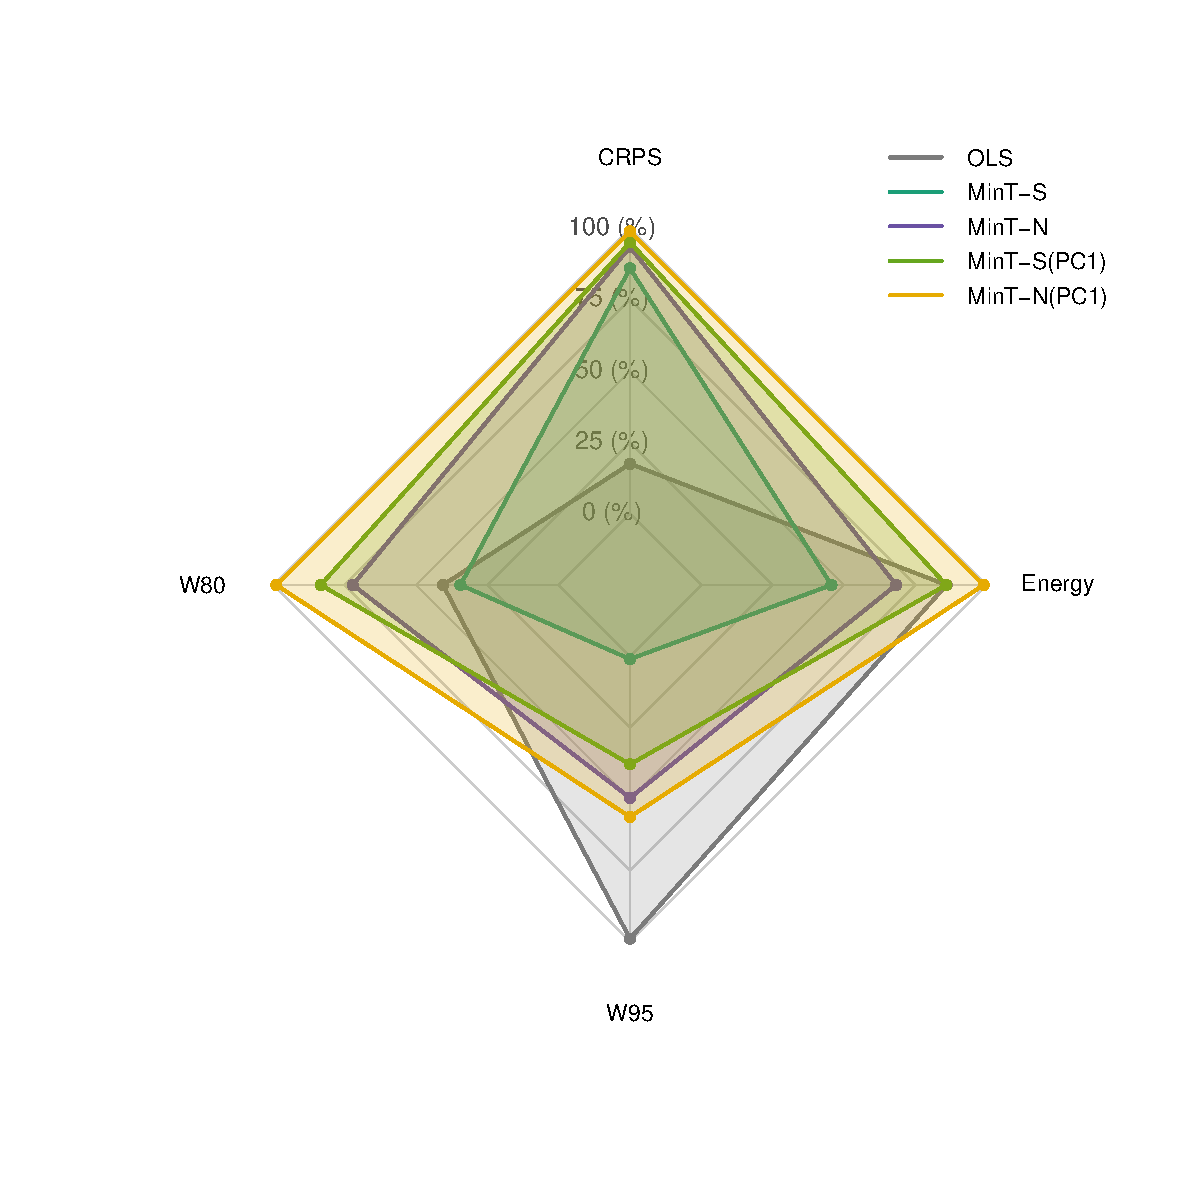
\includegraphics[width=0.7\linewidth,height=\textheight,keepaspectratio]{paper_draft_files/figure-pdf/fig-tourism-radar-1.pdf}

}

\caption{\label{fig-tourism-radar}Radar plot of relative improvements in
probabilistic scores (Winkler score at 80\% and 95\% intervals, CRPS,
and Energy) over the base forecasts. The scores are scaled to a range of
0 to 100, with larger values indicating better performance. The
outermost polygon represents the best possible score (100) and the
innermost polygon represents the worst possible score (0). Only the top
4 MinT approaches are shown, together with the base forecasts.}

\end{figure}%

The summary radar graph in Figure~\ref{fig-tourism-radar} consolidates
these findings. Among the selected MinT variants considering
probabilistic criteria, \emph{MinT-N(PC1)} (yellow polygon) clearly
leads across CRPS, Winkler score at 80\% and 95\% intervals, and Energy
score, extending the improvements seen in the single-metric panels.
Except for the Winkler score at 95\% interval, all MinT variants
outperform the base forecasts.

\section{Conclusions and Future Work}\label{sec-conclusion}

This paper tackles a central bottleneck in Minimum Trace (MinT)
reconciliation: obtaining reliable, positive-definite estimates of the
base-forecast error covariance. The original practice, following
Wickramasuriya et al. (\citeproc{ref-Wickramasuriya2019-xq}{2019}),
estimates the one-step covariance via diagonal-target shrinkage and
obtains multi-step horizons by proportional scaling. We identified three
limitations of this approach--uniform shrinkage, lack of factor
awareness, and horizon-invariant dependence--and proposed alternatives
that address them individually and in combination. Specifically, we
adopt NOVELIST to introduce a more flexible shrinkage target; develop
PC-adjusted variants of shrinkage and NOVELIST to preserve dominant
latent components in the data; and consider multi-step covariance
constructions that relax proportional scaling assumption.

Empirical evidence from Australian domestic tourism yields several
insights. For point reconciliation, shrinkage (and its PC-adjusted
version) remains a robust default choice, while NOVELIST demonstrates
improved performance for probabilistic forecasts. Across both settings,
adjusting for a single dominant principal component consistently
enhances performance, indicating its utility when such latent structures
are present. More complex adjustments, such as incorporating multiple
principal components or horizon-specific covariances, tend to introduce
additional idiosyncratic noise without notable benefits.

Several limitations and directions for future work remain. First, more
intricate simulation designs are needed to further highlight the
differences between shrinkage and NOVELIST, particularly under explicit
factor models and varying sparsity/noise levels. Second, our current
PC-adjusted implementations do not standardise series prior to factor
extraction, which may lead to higher-level series largely influencing
the principal components. Third, we can explore alternative methods that
leverage cross-series information or eigenvalue/eigenvector structures.
Fourth, the observed inferior performance of MinT with shrinkage under
the Winkler 95\% score at higher aggregation levels needs detailed
investigation. Finally, evaluating genuinely \(h\)-step probabilistic
reconciliation remains an open avenue, including how to best regularise
multi-step covariances given limited effective samples.

All data generation, covariance estimation, and reconciliation routines
were implemented in the ReconCov R package and is available under an
open‐source license on GitHub (\citeproc{ref-ReconCov}{Su, 2025}).

\pagebreak

\section{Appendix}\label{sec-appendix}

\subsection{Appendix: Simulation
Supplementary}\label{sec-sim-supplement}

\subsection{Appendix: Australian Domestic Tourism Geographical
Hierarchy}\label{sec-tourism-supplement}

\begingroup\fontsize{8}{10}\selectfont

\begin{longtable}[t]{rllrll}

\caption{\label{tbl-tourism-geo}Geographical divisions of Australia.}

\tabularnewline

\toprule
Series & Name & Label & Series & Name & Label\\
\midrule
1 & Australia & Total & 57 & Bundaberg & CAA\\
2 & NSW & A & 58 & Capricorn & CAB\\
3 & NT & B & 59 & Fraser Coast & CAC\\
4 & QLD & C & 60 & Gladstone & CAD\\
5 & SA & D & 61 & Mackay & CAE\\
\addlinespace
6 & TAS & E & 62 & Southern Queensland Country & CAF\\
7 & VIC & F & 63 & Outback Queensland & CBA\\
8 & WA & G & 64 & Brisbane & CCA\\
9 & ACT & AA & 65 & Gold Coast & CCB\\
10 & Metro NSW & AB & 66 & Sunshine Coast & CCC\\
\addlinespace
11 & Nth Coast NSW & AC & 67 & Townsville & CDA\\
12 & Nth NSW & AD & 68 & Tropical North Queensland & CDB\\
13 & Sth Coast NSW & AE & 69 & Whitsundays & CDC\\
14 & Sth NSW & AF & 70 & Clare Valley & DAA\\
15 & Central NT & BA & 71 & Flinders Ranges and Outback & DAB\\
\addlinespace
16 & Nth Coast NT & BB & 72 & Murray River, Lakes and Coorong & DAC\\
17 & Central Coast QLD & CA & 73 & Riverland & DAD\\
18 & Inland QLD & CB & 74 & Adelaide & DBA\\
19 & Metro QLD & CC & 75 & Adelaide Hills & DBB\\
20 & Nth Coast QLD & CD & 76 & Barossa & DBC\\
\addlinespace
21 & Inland SA & DA & 77 & Fleurieu Peninsula & DCA\\
22 & Metro SA & DB & 78 & Kangaroo Island & DCB\\
23 & Sth Coast SA & DC & 79 & Limestone Coast & DCC\\
24 & West Coast SA & DD & 80 & Eyre Peninsula & DDA\\
25 & Nth East TAS & EA & 81 & Yorke Peninsula & DDB\\
\addlinespace
26 & Nth West TAS & EB & 82 & East Coast & EAA\\
27 & Sth TAS & EC & 83 & Launceston and the North & EAB\\
28 & East Coast VIC & FA & 84 & North West & EBA\\
29 & Metro VIC & FB & 85 & West Coast & EBB\\
30 & Nth East VIC & FC & 86 & Hobart and the South & ECA\\
\addlinespace
31 & Nth West VIC & FD & 87 & Gippsland & FAA\\
32 & West Coast VIC & FE & 88 & Lakes & FAB\\
33 & Nth WA & GA & 89 & Phillip Island & FAC\\
34 & Sth WA & GB & 90 & Geelong and the Bellarine & FBA\\
35 & West Coast WA & GC & 91 & Melbourne & FBB\\
\addlinespace
36 & Canberra & AAA & 92 & Peninsula & FBC\\
37 & Central Coast & ABA & 93 & Central Murray & FCA\\
38 & Sydney & ABB & 94 & Goulburn & FCB\\
39 & Hunter & ACA & 95 & High Country & FCC\\
40 & North Coast NSW & ACB & 96 & Melbourne East & FCD\\
\addlinespace
41 & Blue Mountains & ADA & 97 & Murray East & FCE\\
42 & Central NSW & ADB & 98 & Upper Yarra & FCF\\
43 & New England North West & ADC & 99 & Ballarat & FDA\\
44 & Outback NSW & ADD & 100 & Bendigo Loddon & FDB\\
45 & South Coast & AEA & 101 & Central Highlands & FDC\\
\addlinespace
46 & Capital Country & AFA & 102 & Macedon & FDD\\
47 & Riverina & AFB & 103 & Mallee & FDE\\
48 & Snowy Mountains & AFC & 104 & Spa Country & FDF\\
49 & The Murray & AFD & 105 & Western Grampians & FDG\\
50 & Alice Springs & BAA & 106 & Wimmera & FDH\\
\addlinespace
51 & Barkly & BAB & 107 & Great Ocean Road & FEA\\
52 & Lasseter & BAC & 108 & Australia's North West & GAA\\
53 & MacDonnell & BAD & 109 & Australia's Golden Outback & GBA\\
54 & Darwin & BBA & 110 & Australia's Coral Coast & GCA\\
55 & Katherine Daly & BBB & 111 & Australia's South West & GCB\\
\addlinespace
56 & Litchfield Kakadu Arnhem & BBC & 112 & Destination Perth & GCC\\
\bottomrule

\end{longtable}

\endgroup{}

\pagebreak

\section*{References}\label{references}
\addcontentsline{toc}{section}{References}

\phantomsection\label{refs}
\begin{CSLReferences}{1}{0}
\bibitem[\citeproctext]{ref-Angam2025-od}
Angam, B., Beretta, A., De Poorter, E., Duvinage, M., \& Peralta, D.
(2025). Forecast reconciliation for vaccine supply chain optimization.
In \emph{Communications in computer and information science} (pp.
101--118). Springer Nature Switzerland.
\url{https://doi.org/10.1007/978-3-031-74650-5/_6}

\bibitem[\citeproctext]{ref-Athanasopoulos2009-lp}
Athanasopoulos, G., Ahmed, R. A., \& Hyndman, R. J. (2009). Hierarchical
forecasts for australian domestic tourism. \emph{International Journal
of Forecasting}, \emph{25}(1), 146--166.
\url{https://doi.org/10.1016/j.ijforecast.2008.07.004}

\bibitem[\citeproctext]{ref-Athanasopoulos2024-as}
Athanasopoulos, G., Hyndman, R. J., Kourentzes, N., \& Panagiotelis, A.
(2024). \emph{Forecast reconciliation: A review}. \emph{40}(2),
430--456.
\url{https://www.sciencedirect.com/science/article/pii/S0169207023001097}

\bibitem[\citeproctext]{ref-Ben-Taieb2019-yx}
Ben Taieb, S., \& Koo, B. (2019). Regularized regression for
hierarchical forecasting without unbiasedness conditions.
\emph{Proceedings of the 25th ACM SIGKDD International Conference on
Knowledge Discovery \& Data Mining}.
\url{https://doi.org/10.1145/3292500.3330976}

\bibitem[\citeproctext]{ref-Ben-Taieb2021-bn}
Ben Taieb, S., Taylor, J. W., \& Hyndman, R. J. (2021). Hierarchical
probabilistic forecasting of electricity demand with smart meter data.
\emph{Journal of the American Statistical Association}, \emph{116}(533),
27--43. \url{https://doi.org/10.1080/01621459.2020.1736081}

\bibitem[\citeproctext]{ref-Bickel2008-nh}
Bickel, P. J., \& Levina, E. (2008). Covariance regularization by
thresholding. \emph{Annals of Statistics}, \emph{36}(6), 2577--2604.
\url{https://doi.org/10.1214/08-aos600}

\bibitem[\citeproctext]{ref-Cai2011-jf}
Cai, T., \& Liu, W. (2011). Adaptive thresholding for sparse covariance
matrix estimation. \emph{Journal of the American Statistical
Association}, \emph{106}(494), 672--684.
\url{https://doi.org/10.1198/jasa.2011.tm10560}

\bibitem[\citeproctext]{ref-Carrara2025-rz}
Carrara, C., Zambon, L., Azzimonti, D., \& Corani, G. (2025). A novel
shrinkage estimator of the covariance matrix for hierarchical time
series. In \emph{Italian statistical society series on advances in
statistics} (pp. 140--145). Springer Nature Switzerland.
\url{https://doi.org/10.1007/978-3-031-96736-8/_24}

\bibitem[\citeproctext]{ref-Di-Modica2021-ad}
Di Modica, C., Pinson, P., \& Ben Taieb, S. (2021). Online forecast
reconciliation in wind power prediction. \emph{Electric Power Systems
Research}, \emph{190}(106637), 106637.
\url{https://doi.org/10.1016/j.epsr.2020.106637}

\bibitem[\citeproctext]{ref-El-Gemayel2022-hx}
El Gemayel, J., Lafarguette, R., Itd, K. M., et al. (2022). \emph{United
arab emirates: Technical assistance reportliquidity management and
forecasting}.

\bibitem[\citeproctext]{ref-Van_Erven2015-nx}
Erven, T. van, \& Cugliari, J. (2015). Game-theoretically optimal
reconciliation of contemporaneous hierarchical time series forecasts. In
\emph{Modeling and stochastic learning for forecasting in high
dimensions} (pp. 297--317). Springer International Publishing.
\url{https://doi.org/10.1007/978-3-319-18732-7/_15}

\bibitem[\citeproctext]{ref-Fan2013-jz}
Fan, J., Liao, Y., \& Mincheva, M. (2013). Large covariance estimation
by thresholding principal orthogonal complements. \emph{Journal of the
Royal Statistical Society. Series B, Statistical Methodology},
\emph{75}(4), 603--680. \url{https://doi.org/10.1111/rssb.12016}

\bibitem[\citeproctext]{ref-Gamakumara2020-ml}
Gamakumara, P. (2020). \emph{Probabilistic forecast reconciliation:
Theory and applications} {[}PhD thesis, Monash University{]}.
\url{https://doi.org/10.26180/5e4ca9d0c4b9d}

\bibitem[\citeproctext]{ref-Hardin2013-wu}
Hardin, J., Garcia, S. R., \& Golan, D. (2013). A method for generating
realistic correlation matrices. \emph{The Annals of Applied Statistics},
\emph{7}(3), 1733--1762. \url{https://www.jstor.org/stable/23566492}

\bibitem[\citeproctext]{ref-Higham2002-te}
Higham, N. (2002). Computing the nearest correlation matrix---a problem
from finance. \emph{Ima Journal of Numerical Analysis}, \emph{22},
329--343. \url{https://doi.org/10.1093/IMANUM/22.3.329}

\bibitem[\citeproctext]{ref-Huang2019-ua}
Huang, N., \& Fryzlewicz, P. (2019). {NOVELIST} estimator of large
correlation and covariance matrices and their inverses. \emph{Test
(Madrid, Spain)}, \emph{28}(3), 694--727.
\url{https://doi.org/10.1007/s11749-018-0592-4}

\bibitem[\citeproctext]{ref-Hyndman2011-jv}
Hyndman, R. J., Ahmed, R. A., Athanasopoulos, G., \& Shang, H. L.
(2011). Optimal combination forecasts for hierarchical time series.
\emph{Computational Statistics \& Data Analysis}, \emph{55}(9),
2579--2589. \url{https://doi.org/10.1016/j.csda.2011.03.006}

\bibitem[\citeproctext]{ref-Hyndman2008-rf}
Hyndman, R. J., \& Khandakar, Y. (2008). Automatic time series
forecasting: The forecast package for {R}. \emph{Journal of Statistical
Software}, \emph{27}, 1--22. \url{https://doi.org/10.18637/JSS.V027.I03}

\bibitem[\citeproctext]{ref-Hyndman2016-ic}
Hyndman, R. J., Lee, A. J., \& Wang, E. (2016). Fast computation of
reconciled forecasts for hierarchical and grouped time series.
\emph{Computational Statistics \& Data Analysis}, \emph{97}, 16--32.
\url{https://doi.org/10.1016/j.csda.2015.11.007}

\bibitem[\citeproctext]{ref-Jeon2019-wm}
Jeon, J., Panagiotelis, A., \& Petropoulos, F. (2019). Probabilistic
forecast reconciliation with applications to wind power and electric
load. \emph{European Journal of Operational Research}, \emph{279}(2),
364--379. \url{https://doi.org/10.1016/j.ejor.2019.05.020}

\bibitem[\citeproctext]{ref-Ledoit2012-ga}
Ledoit, O., \& Wolf, M. (2012). Nonlinear shrinkage estimation of
large-dimensional covariance matrices. \emph{Annals of Statistics}.
\url{https://doi.org/10.1214/12-AOS989}

\bibitem[\citeproctext]{ref-Ledoit2020-xt}
Ledoit, O., \& Wolf, M. (2020). Analytical nonlinear shrinkage of
large-dimensional covariance matrices. \emph{Annals of Statistics},
\emph{48}(5), 3043--3065. \url{https://doi.org/10.1214/19-AOS1921}

\bibitem[\citeproctext]{ref-Li2019-vv}
Li, H., Li, H., Lu, Y., \& Panagiotelis, A. (2019). A forecast
reconciliation approach to cause-of-death mortality modeling.
\emph{Insurance, Mathematics \& Economics}, \emph{86}, 122--133.
\url{https://doi.org/10.1016/j.insmatheco.2019.02.011}

\bibitem[\citeproctext]{ref-Nixtla}
Nixtla. (2025). \emph{Time series forecasting software}.
\url{https://www.nixtla.io/}

\bibitem[\citeproctext]{ref-O-Hara-Wild2024-we}
O'Hara-Wild, M., Hyndman, R. J., \& Wang, E. (2024). \emph{Fabletools
{R} package} (Version v0.5.0). \url{https://fabletools.tidyverts.org/}

\bibitem[\citeproctext]{ref-Panagiotelis2023-fs}
Panagiotelis, A., Gamakumara, P., Athanasopoulos, G., \& Hyndman, R. J.
(2023). Probabilistic forecast reconciliation: Properties, evaluation
and score optimisation. \emph{European Journal of Operational Research},
\emph{306}(2), 693--706.
\url{https://doi.org/10.1016/j.ejor.2022.07.040}

\bibitem[\citeproctext]{ref-Rothman2009-yf}
Rothman, A. J., Levina, E., \& Zhu, J. (2009). Generalized thresholding
of large covariance matrices. \emph{Journal of the American Statistical
Association}, \emph{104}(485), 177--186.
\url{https://doi.org/10.1198/jasa.2009.0101}

\bibitem[\citeproctext]{ref-Schafer2005-yw}
Schäfer, J., \& Strimmer, K. (2005). A shrinkage approach to large-scale
covariance matrix estimation and implications for functional genomics.
\emph{Statistical Applications in Genetics and Molecular Biology},
\emph{4}(1), Article32. \url{https://doi.org/10.2202/1544-6115.1175}

\bibitem[\citeproctext]{ref-Seaman2022-bb}
Seaman, B., \& Bowman, J. (2022). Applicability of the {M5} to
forecasting at walmart. \emph{International Journal of Forecasting},
\emph{38}(4), 1468--1472.
\url{https://doi.org/10.1016/j.ijforecast.2021.06.002}

\bibitem[\citeproctext]{ref-Shang2017-ux}
Shang, H. L., \& Hyndman, R. J. (2017). Grouped functional time series
forecasting: An application to age-specific mortality rates.
\emph{Journal of Computational and Graphical Statistics: A Joint
Publication of American Statistical Association, Institute of
Mathematical Statistics, Interface Foundation of North America},
\emph{26}(2), 330--343.
\url{https://doi.org/10.1080/10618600.2016.1237877}

\bibitem[\citeproctext]{ref-ReconCov}
Su, V. (2025). \emph{{ReconCov} {R} package} (Version beta).
\url{https://github.com/lordtahdus/ReconCov}

\bibitem[\citeproctext]{ref-tourism-au}
\emph{Tourism research australia}. (2024).
\url{https://www.tra.gov.au/}.

\bibitem[\citeproctext]{ref-Wickramasuriya2024-mb}
Wickramasuriya, S. L. (2024). Probabilistic forecast reconciliation
under the gaussian framework. \emph{Journal of Business \& Economic
Statistics: A Publication of the American Statistical Association},
\emph{42}(1), 272--285.
\url{https://doi.org/10.1080/07350015.2023.2181176}

\bibitem[\citeproctext]{ref-Wickramasuriya2019-xq}
Wickramasuriya, S. L., Athanasopoulos, G., \& Hyndman, R. J. (2019).
Optimal forecast reconciliation for hierarchical and grouped time series
through trace minimization. \emph{Journal of the American Statistical
Association}, \emph{114}(526), 804--819.
\url{https://doi.org/10.1080/01621459.2018.1448825}

\bibitem[\citeproctext]{ref-Wickramasuriya2020-uk}
Wickramasuriya, S. L., Turlach, B. A., \& Hyndman, R. J. (2020). Optimal
non-negative forecast reconciliation. \emph{Statistics and Computing},
\emph{30}(5), 1167--1182.
\url{https://doi.org/10.1007/s11222-020-09930-0}

\end{CSLReferences}




\end{document}
